\documentclass[a4paper, 11pt]{article} % Font size (can be 10pt, 11pt or 12pt)

\usepackage[protrusion=true,expansion=true]{microtype} % Better typography
\usepackage{graphicx, grffile} % Required for including pictures
\usepackage{hyperref} % Clickable cross-referencing

\usepackage{mathpazo} % Use the Palatino font
\usepackage{amsmath} % Gets \text{} working in math mode.
\usepackage[T1]{fontenc} % Required for accented characters
\linespread{2} % Change line spacing here, Palatino benefits from a slight increase by default
\usepackage[margin=1.5in]{geometry}
\usepackage{changepage}
\usepackage{collectbox}
\usepackage{float}

\makeatletter
\newcommand{\sqbox}{%
	\collectbox{%
		\@tempdima=\dimexpr\width-\totalheight\relax
		\ifdim\@tempdima<\z@
		\fbox{\hbox{\hspace{-.5\@tempdima}\BOXCONTENT\hspace{-.5\@tempdima}}}%
		\else
		\ht\collectedbox=\dimexpr\ht\collectedbox+.5\@tempdima\relax
		\dp\collectedbox=\dimexpr\dp\collectedbox+.5\@tempdima\relax
		\fbox{\BOXCONTENT}%
		\fi
	}%
}
\makeatother

\makeatletter
\renewcommand\@biblabel[1]{\textbf{#1.}} % Change the square brackets for each bibliography item 
%from '[1]' to '1.'
\renewcommand{\@listI}{\itemsep=0pt} % Reduce the space between items in the itemize and 
%enumerate environments and the bibliography
\renewcommand{\sectionautorefname}{\S}

\renewcommand{\maketitle}{
\begin{flushright}
	{\LARGE\@title}
	\vspace{50pt} \\
	{\large\@author}
	\\\@date
	\vspace{40pt}
\end{flushright}
}

\title{
	\begin{figure}
		\begin{center}
					
\includegraphics[width=8cm]{figures/logo.jpg}
		\end{center}
	\end{figure}	
	\textbf{ST3288 UROPS Report
}\\
Applying machine learning techniques to determine the occupancy of parking lots}

\author{\textsc{Rayakar Achal Ajeet, A0156139B}\\
		\texttt{\hyperlink{achal@u.nus.edu}{achal@u.nus.edu}}\\
		\textit{National University of Singapore}
}

\date{7th August, 2018}

%----------------------------------------------------------------------------------------

\begin{document}

\maketitle % Print the title section

\newpage

\tableofcontents

\newpage

\section{Summary}
    This report discusses the conclusion of the two-semester UROPS project entitled ``Parking Lot
    Classification''; namely, it details the suite of tools developed and results achieved in the effort to use
    convolutional neural networks (CNNs) to ascertain the state of a parking lot given its picture. The 
    report will briefly recount the first semester's results, and intentions before delving into how these 
    motivations developed in the second.
\newpage
\section{Recount of ST2288: ``Parking Lot Classification''}
	The motivation behind investigating the use of CNNs in this task was to determine whether it was 
	possible to reliably and inexpensively increase the resolution of information available to drivers 
	looking for parking space; in Singapore, most public parking lots provide users with the number of 
	spots left, but not \textit{where} such spots are. When parking is scarce, traversal to find free spots 
	can be a great inconvenience. Thus, an Internet-of-Things idea based on the usage of 
	already-installed CCTV cameras was proposed to be tested:
	\begin{center}
		\textbf{
			how can one use the \textit{image} of a parking lot to determine its spot-wise occupancy, and 
			then deliver this information to users, in real-time?
		}
	\end{center}
	CNNs were selected to be the classification model behind this idea's implementation since they are 
	currently state-of-the-art for many computer vision tasks.
	The  following was the proposed workflow of a system based on this idea: 
	\begin{enumerate}
		\item User requests for spot-wise occupancy status of a given parking lot through a mobile 
		application created to handle such requests in real-time.
		\item A picture of the lot is taken by a pre-existing CCTV or dedicated camera, and transmitted to 
		the associated cloud-based CNN.
		\item Each spot in the parking lot is classified by this CNN as either empty or occupied.
		\item The picture is then deleted, and the is user sent a spatially-accurate abstraction of 
		spot-wise occupancy status (possibly in the manner pictured below).
	\end{enumerate}
	\begin{figure}[H]
		\centering
		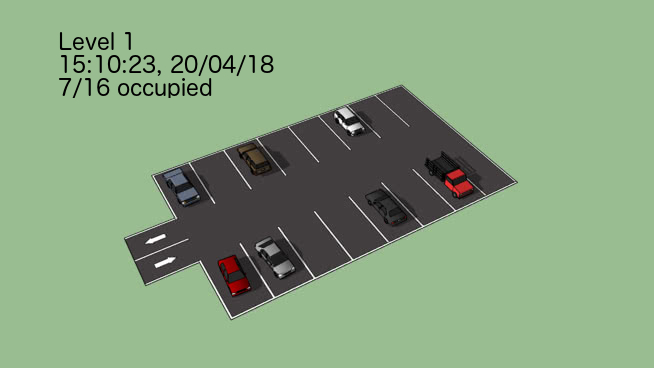
\includegraphics[width=8cm]{figures/mock-up.jpg}
		\caption{This visual could be delivered to users through the mobile application.}
	\end{figure}
	The focus of the previous semester's work was solely the third step of the above workflow: to 
	explore and determine the effectiveness of CNNs for this classification task. To this end, CNNs were 
	found to work very well. A publicly-available parking lot image dataset, \textit{PKLot}, was used to 
	train, validate, and test CNNs created\footnote{This dataset can be found at: 
	\hyperlink{https://web.inf.ufpr.br/vri/databases/parking-lot-database/}
	{web.inf.ufpr.br/vri/databases/parking-lot-database/}}. It comprises of 695,899 images of 
	parking spots taken from two parking lots over the course of about 30 days, in which there was 
	great variation of weather and illumination \cite{pklot-paper}\relax. The following are three example 
	images from this dataset:
	\vskip 5mm
	\begin{figure}[H]
		\centering
		
\includegraphics[width=1cm]{figures/pklot_example_1.jpg}
		\caption{An occupied spot from the first parking lot, in sunshine.}
	\end{figure}
	\begin{figure}[H]
		\centering
		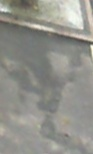
\includegraphics[width=1cm]{figures/pklot_example_2.jpg}
		\caption{An empty spot from one angle of the second parking lot, in overcast conditions.}
		\vspace{5mm}
		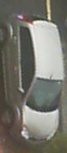
\includegraphics[width=1cm]{figures/pklot_example_3.jpg}
		\caption{An occupied spot from the second angle of the second parking lot, in rain.}
	\end{figure}
	\hspace*{-6mm}The testing accuracies of the CNNs created for each lot in this dataset were greater 
	than 99.8\%, which translates to the misclassification of about 260 spots in requesting for the 
	prediction of the state of about 175,000.The following was their architecture:
	\begin{itemize}
		\setlength\itemsep{-3mm}
		\item[] (Learning rate: 0.001)
		\item[] Input layer: reads in 32-by-32 color images of parking spots.
		\item[] Convolutional layer 1: applies 32 5-by-5 filters, and then the 
		rectified exponential linear unit (ReLU) activation function.
		\item[] Pooling layer 1: performs max pooling with a 2-by-2 filter.
		\item[] Convolutional layer 2: applies 64 3-by-3 filters, and then the 
		ReLU activation function.
		\item[] Pooling layer 2: performs max pooling with a 2-by-2 filter.
		\item[] Fully-connected layer 1: comprises of 1,024 neurons.
		\item[] Output layer: 2 neurons, representing the output vector.
		\vspace*{-4mm}
		\begin{enumerate}
			\setlength\itemsep{-3mm}
			\item[] (0, 1) $\rightarrow$ occupied spot
			\item[] (1, 0) $\rightarrow$ empty spot
		\end{enumerate}
	\end{itemize}
   	The CNNs were implemented using 
   	\href{https://www.tensorflow.org}{TensorFlow}, an efficient and 
   	well-supported deep-learning library written for the Python programming language. Training and 
   	testing of the CNNs was done online on \href{https://www.floydhub.com}{FloydHub}. FloydHub is a 
   	Platform-as-a-Service that quite inexpensively offers a pre-configured programming environment on 
   	powerful hardware for machine learning purposes. Users run ``jobs'' through a command-line client, 
   	with data and algorithms stored on FloydHub. Training metrics and logs can also be automatically 
    generated:
    \vskip 5mm
    \begin{figure}[H]
    	\centering
    	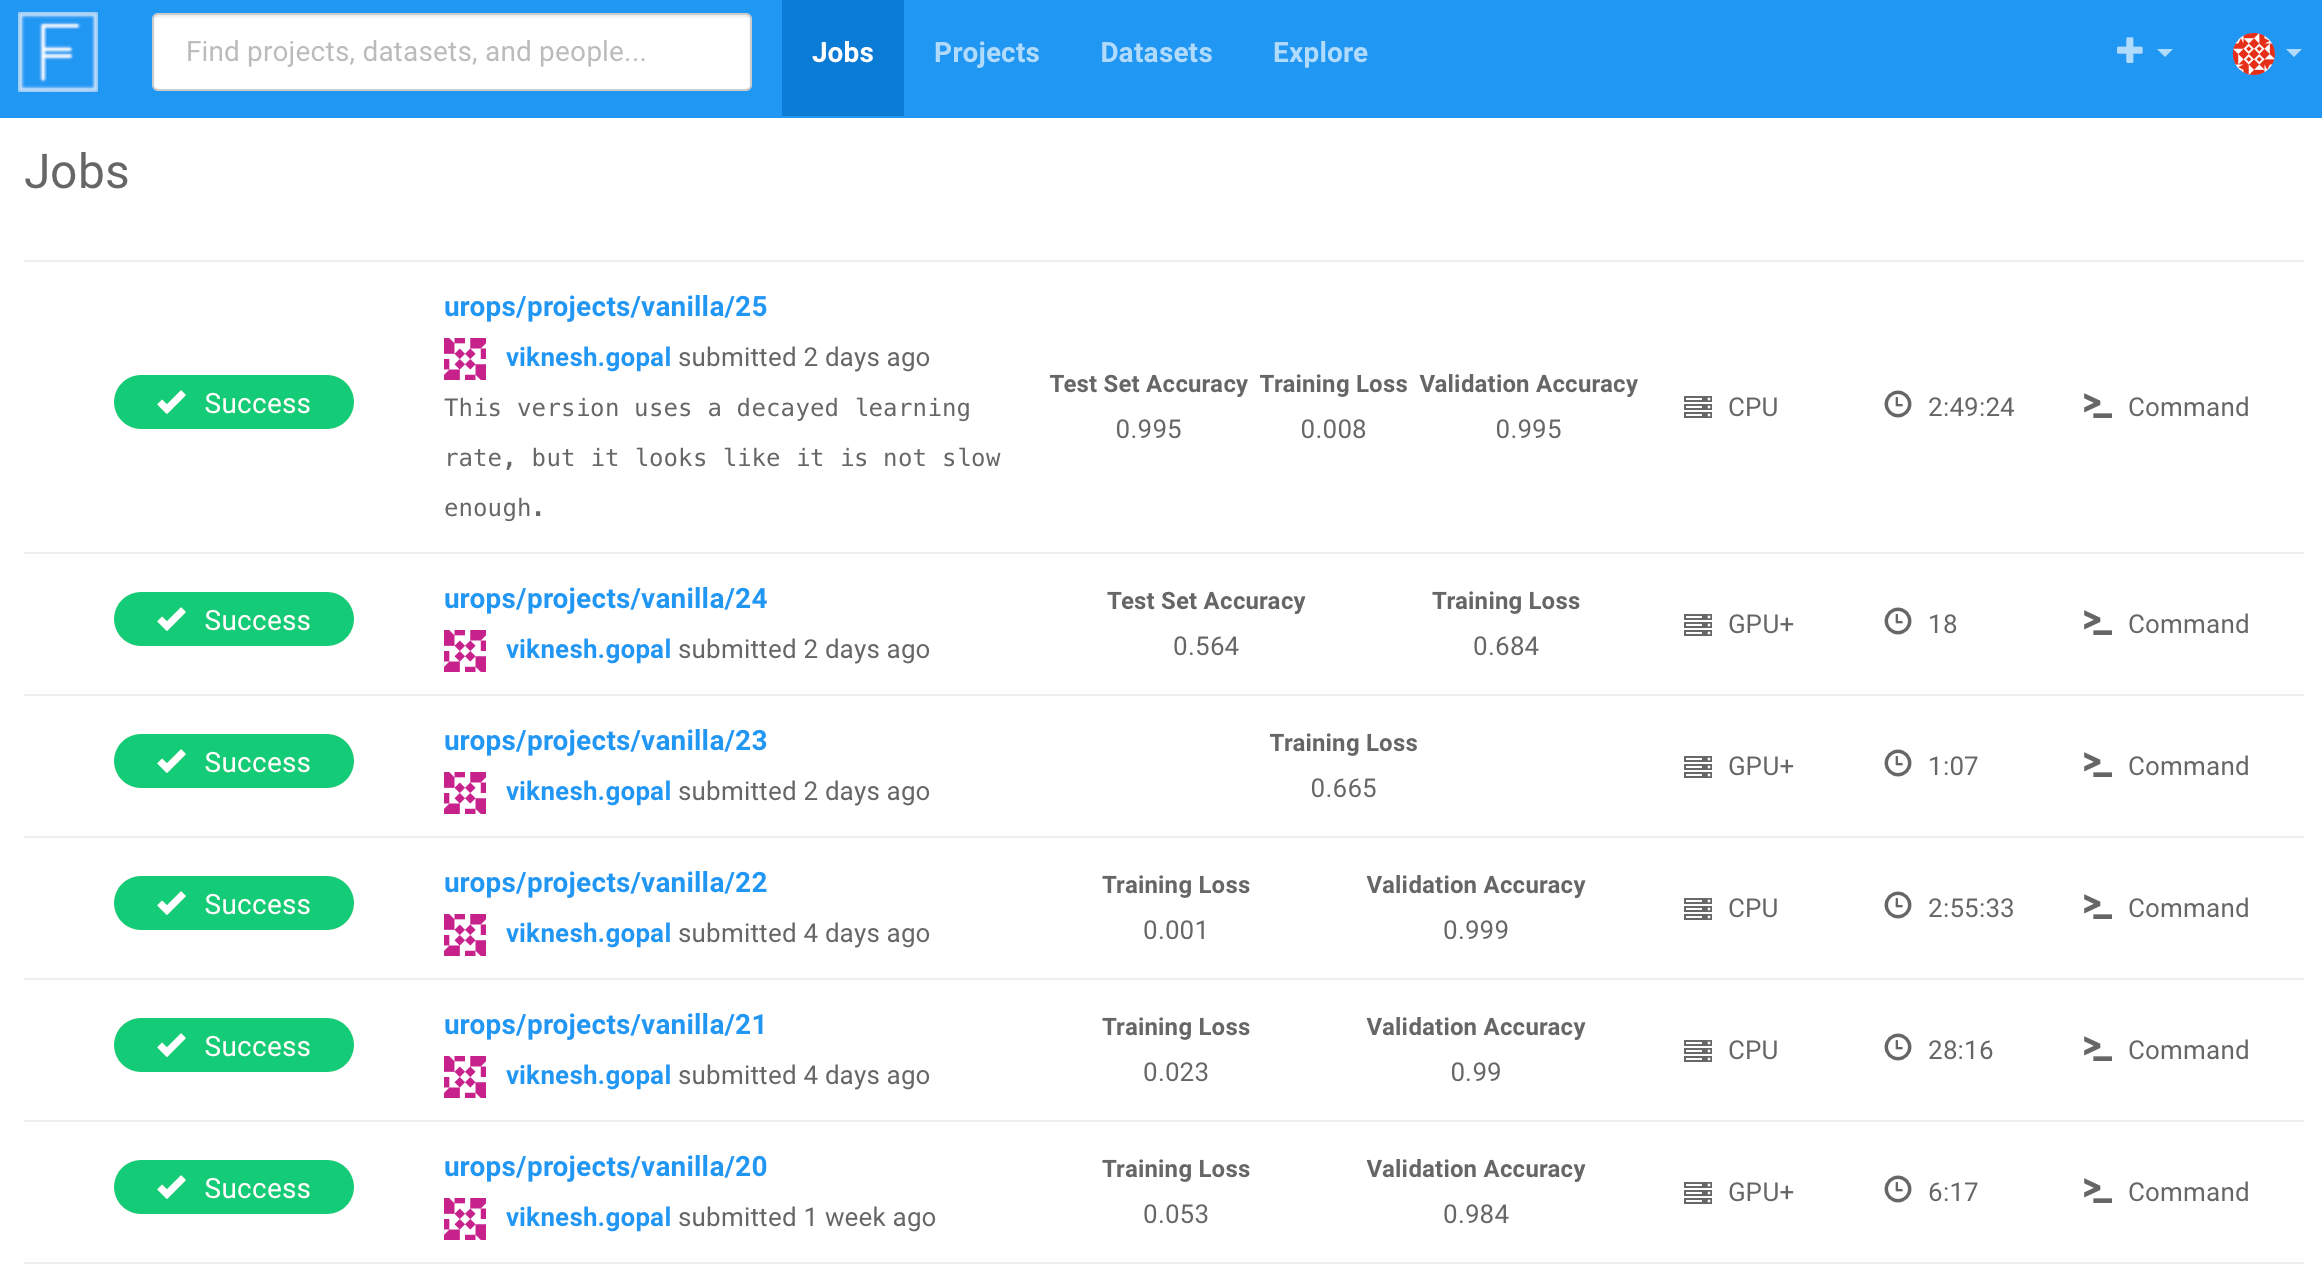
\includegraphics[width=14cm]{figures/floydhub.png}
    	\caption{Log of jobs run on FloydHub.}
    \end{figure}
	\newpage
	With the above results and tools, ST2288 was concluded. This left trialling of the practical 
	application of this idea in the local context to ST3288. The rest of this report details the unique 
	challenges involved in the creation and management of original data, the tools created in response, 
	and the deep generalizability of the resulting CNN-creation workflow to other machine learning 
	projects. The algorithms and files referred to in this report are as they are found on  
	\hyperlink{https://github.com/nurmister/urops}{github.com/nurmister/urops}.
\newpage
\section{Creation of \textit{NUSLot}}
	\subsection{Collection schedule and setup}
		\textit{NUSLot} is the culmination of the data collection, processing, and labeling efforts of this 
		project; it comprises of 50,000 labeled examples of spots of the parking lot belonging to block 
		S17 at the Faculty of Science\footnote{This dataset can be found at: 
		\hyperlink{https://goo.gl/fV2NXS}{goo.gl/fV2NXS}}. The following are three example images 
		from this dataset:
		\vskip 5mm
		\begin{figure}[H]
			\centering
			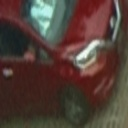
\includegraphics[width=2cm]{figures/nuslot_example_1.jpg}
			\caption{An occupied spot.}
			\vspace{5mm}
			
\includegraphics[width=2cm]{figures/nuslot_example_2.jpg}
			\caption{An empty spot.}
			\vspace{5mm}
			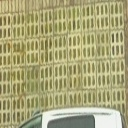
\includegraphics[width=2cm]{figures/nuslot_example_3.jpg}
			\caption{Another empty spot. Notice the occlusion caused by the roof of the vehicle occupying 
			the adjacent spot.}
		\end{figure}
		\hspace*{-6mm}More specifically, this dataset consists of 50,000 128-by-128 pixel BGR images of 
		parking spots, taken between the fourteenth of June and the 24th of July. These images were taken 
		from the following vantage:
		\vskip 5mm
		\begin{figure}[H]
			\centering
			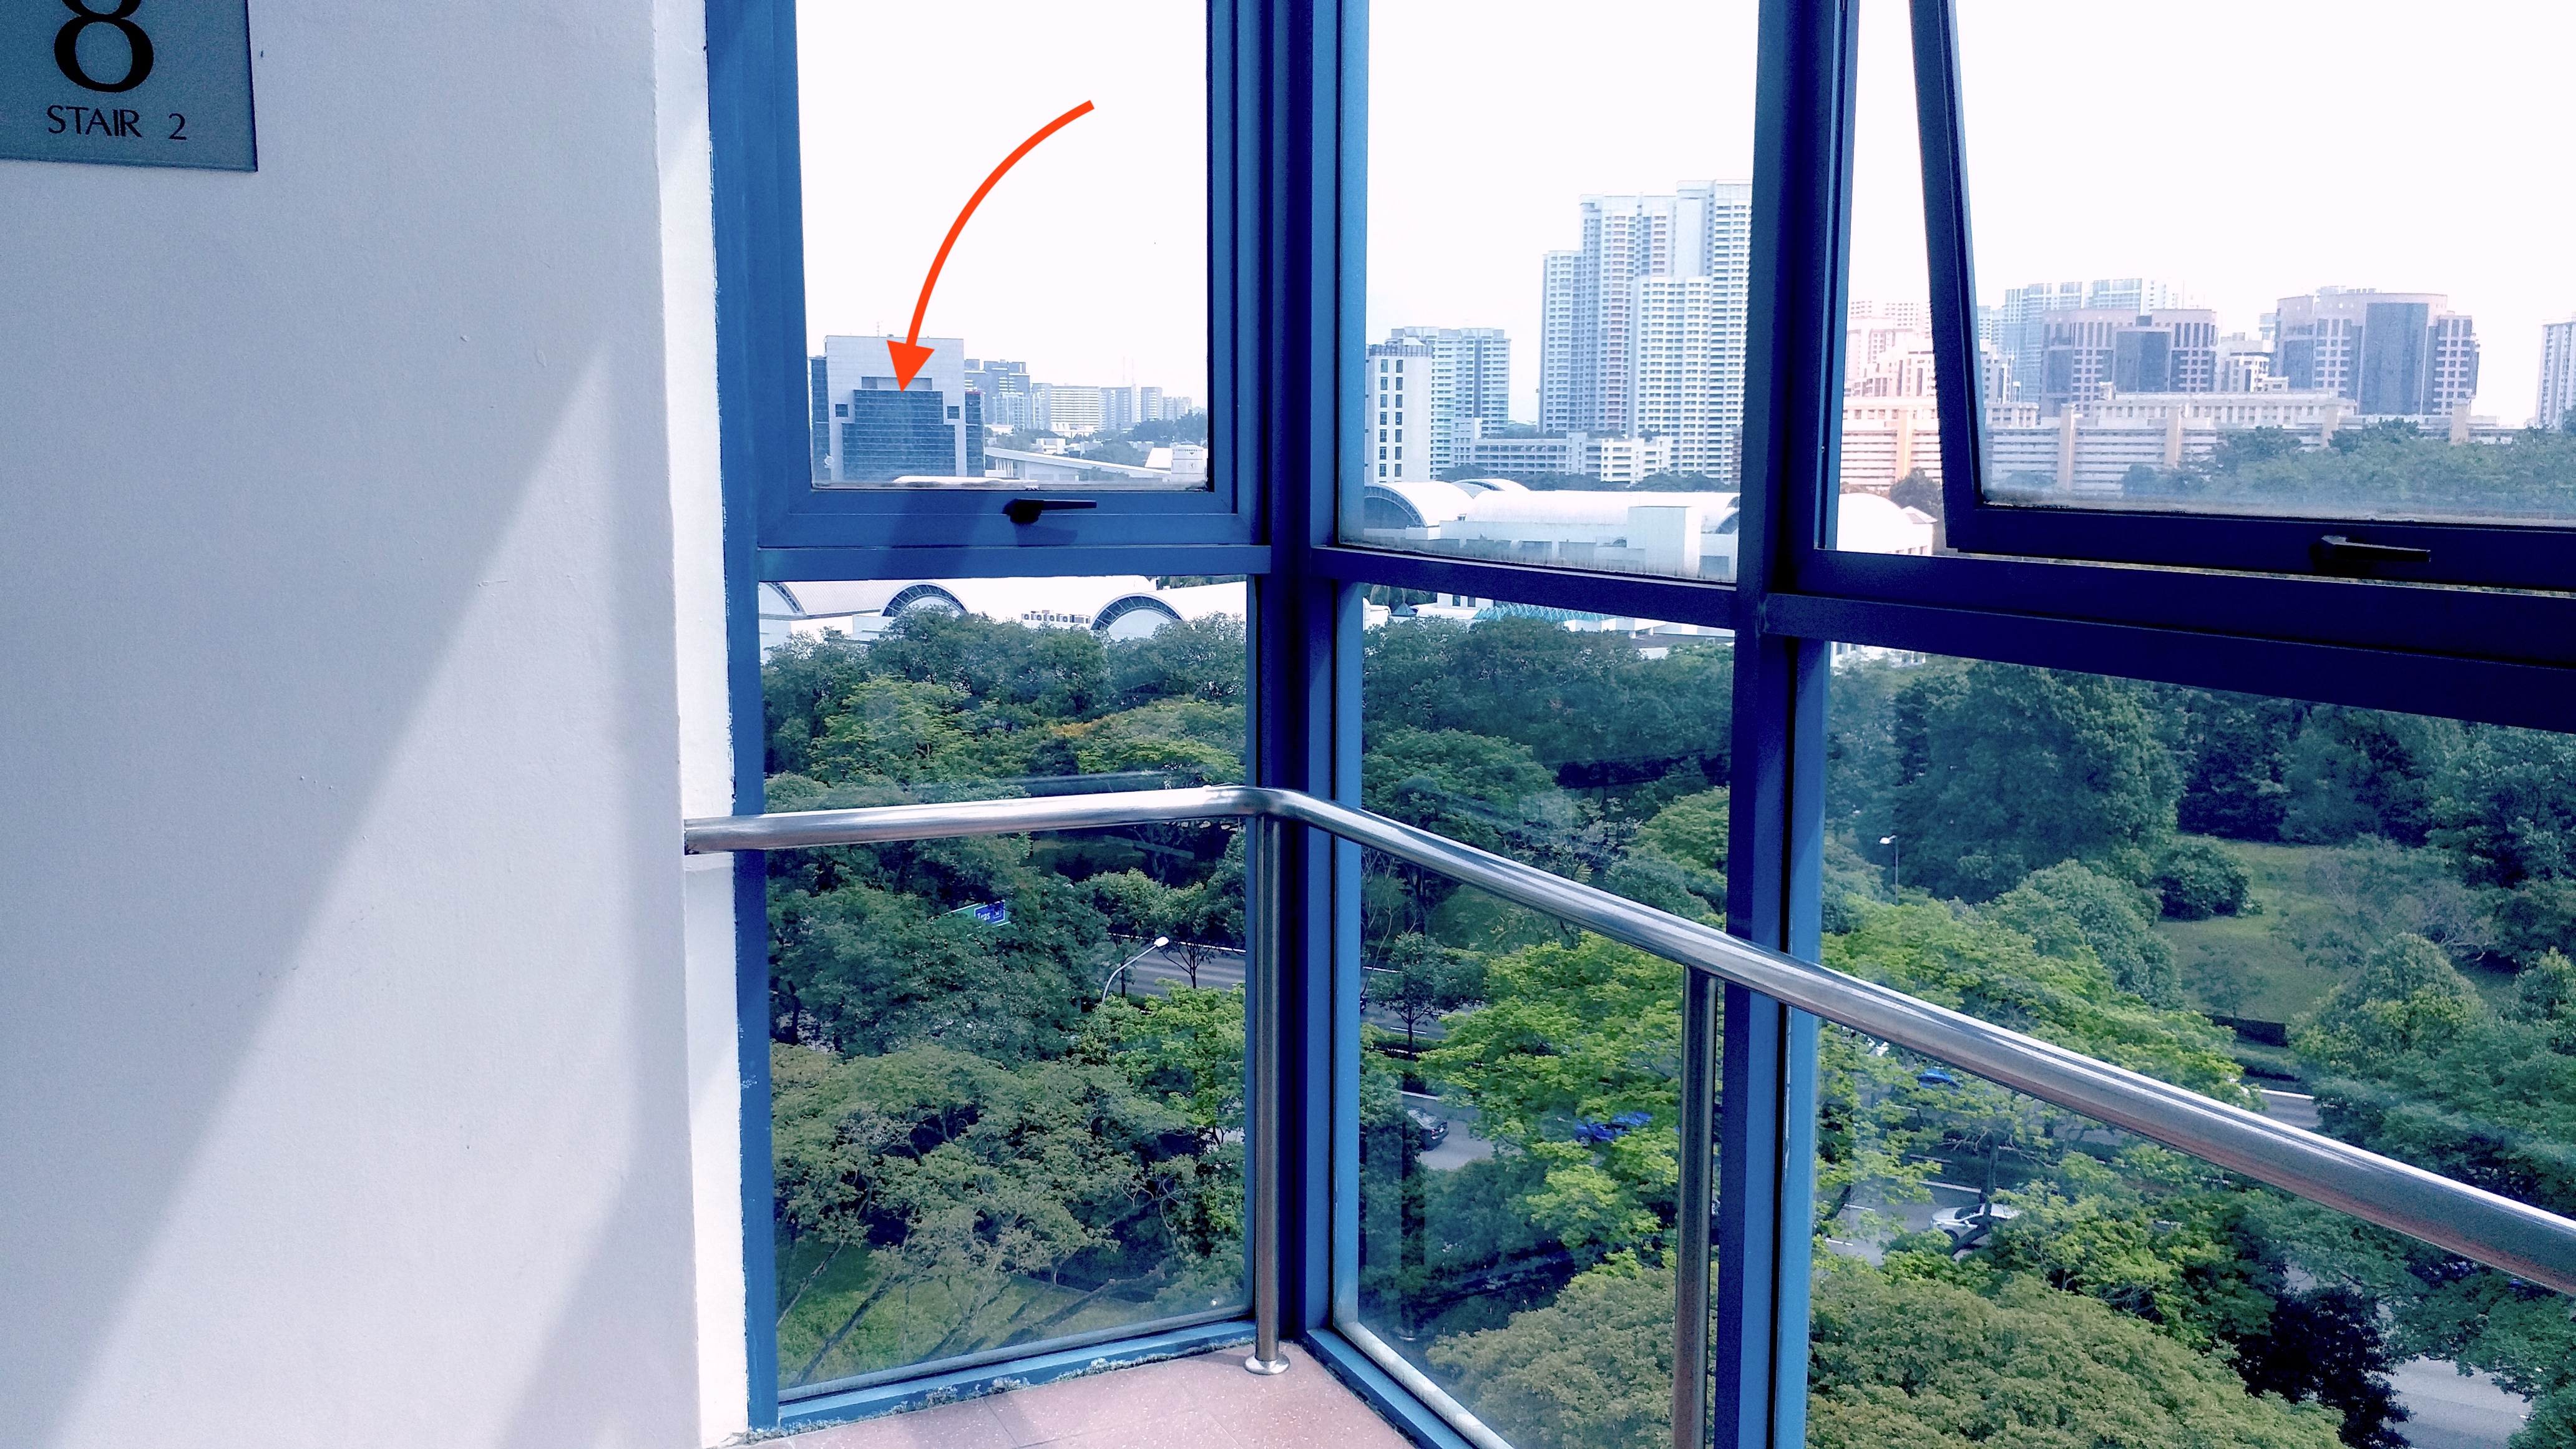
\includegraphics[width=0.5\textwidth]{figures/context_1.jpg}
			\caption{A Raspberry Pi-based camera was mounted on this window,}
			\vskip 5mm
			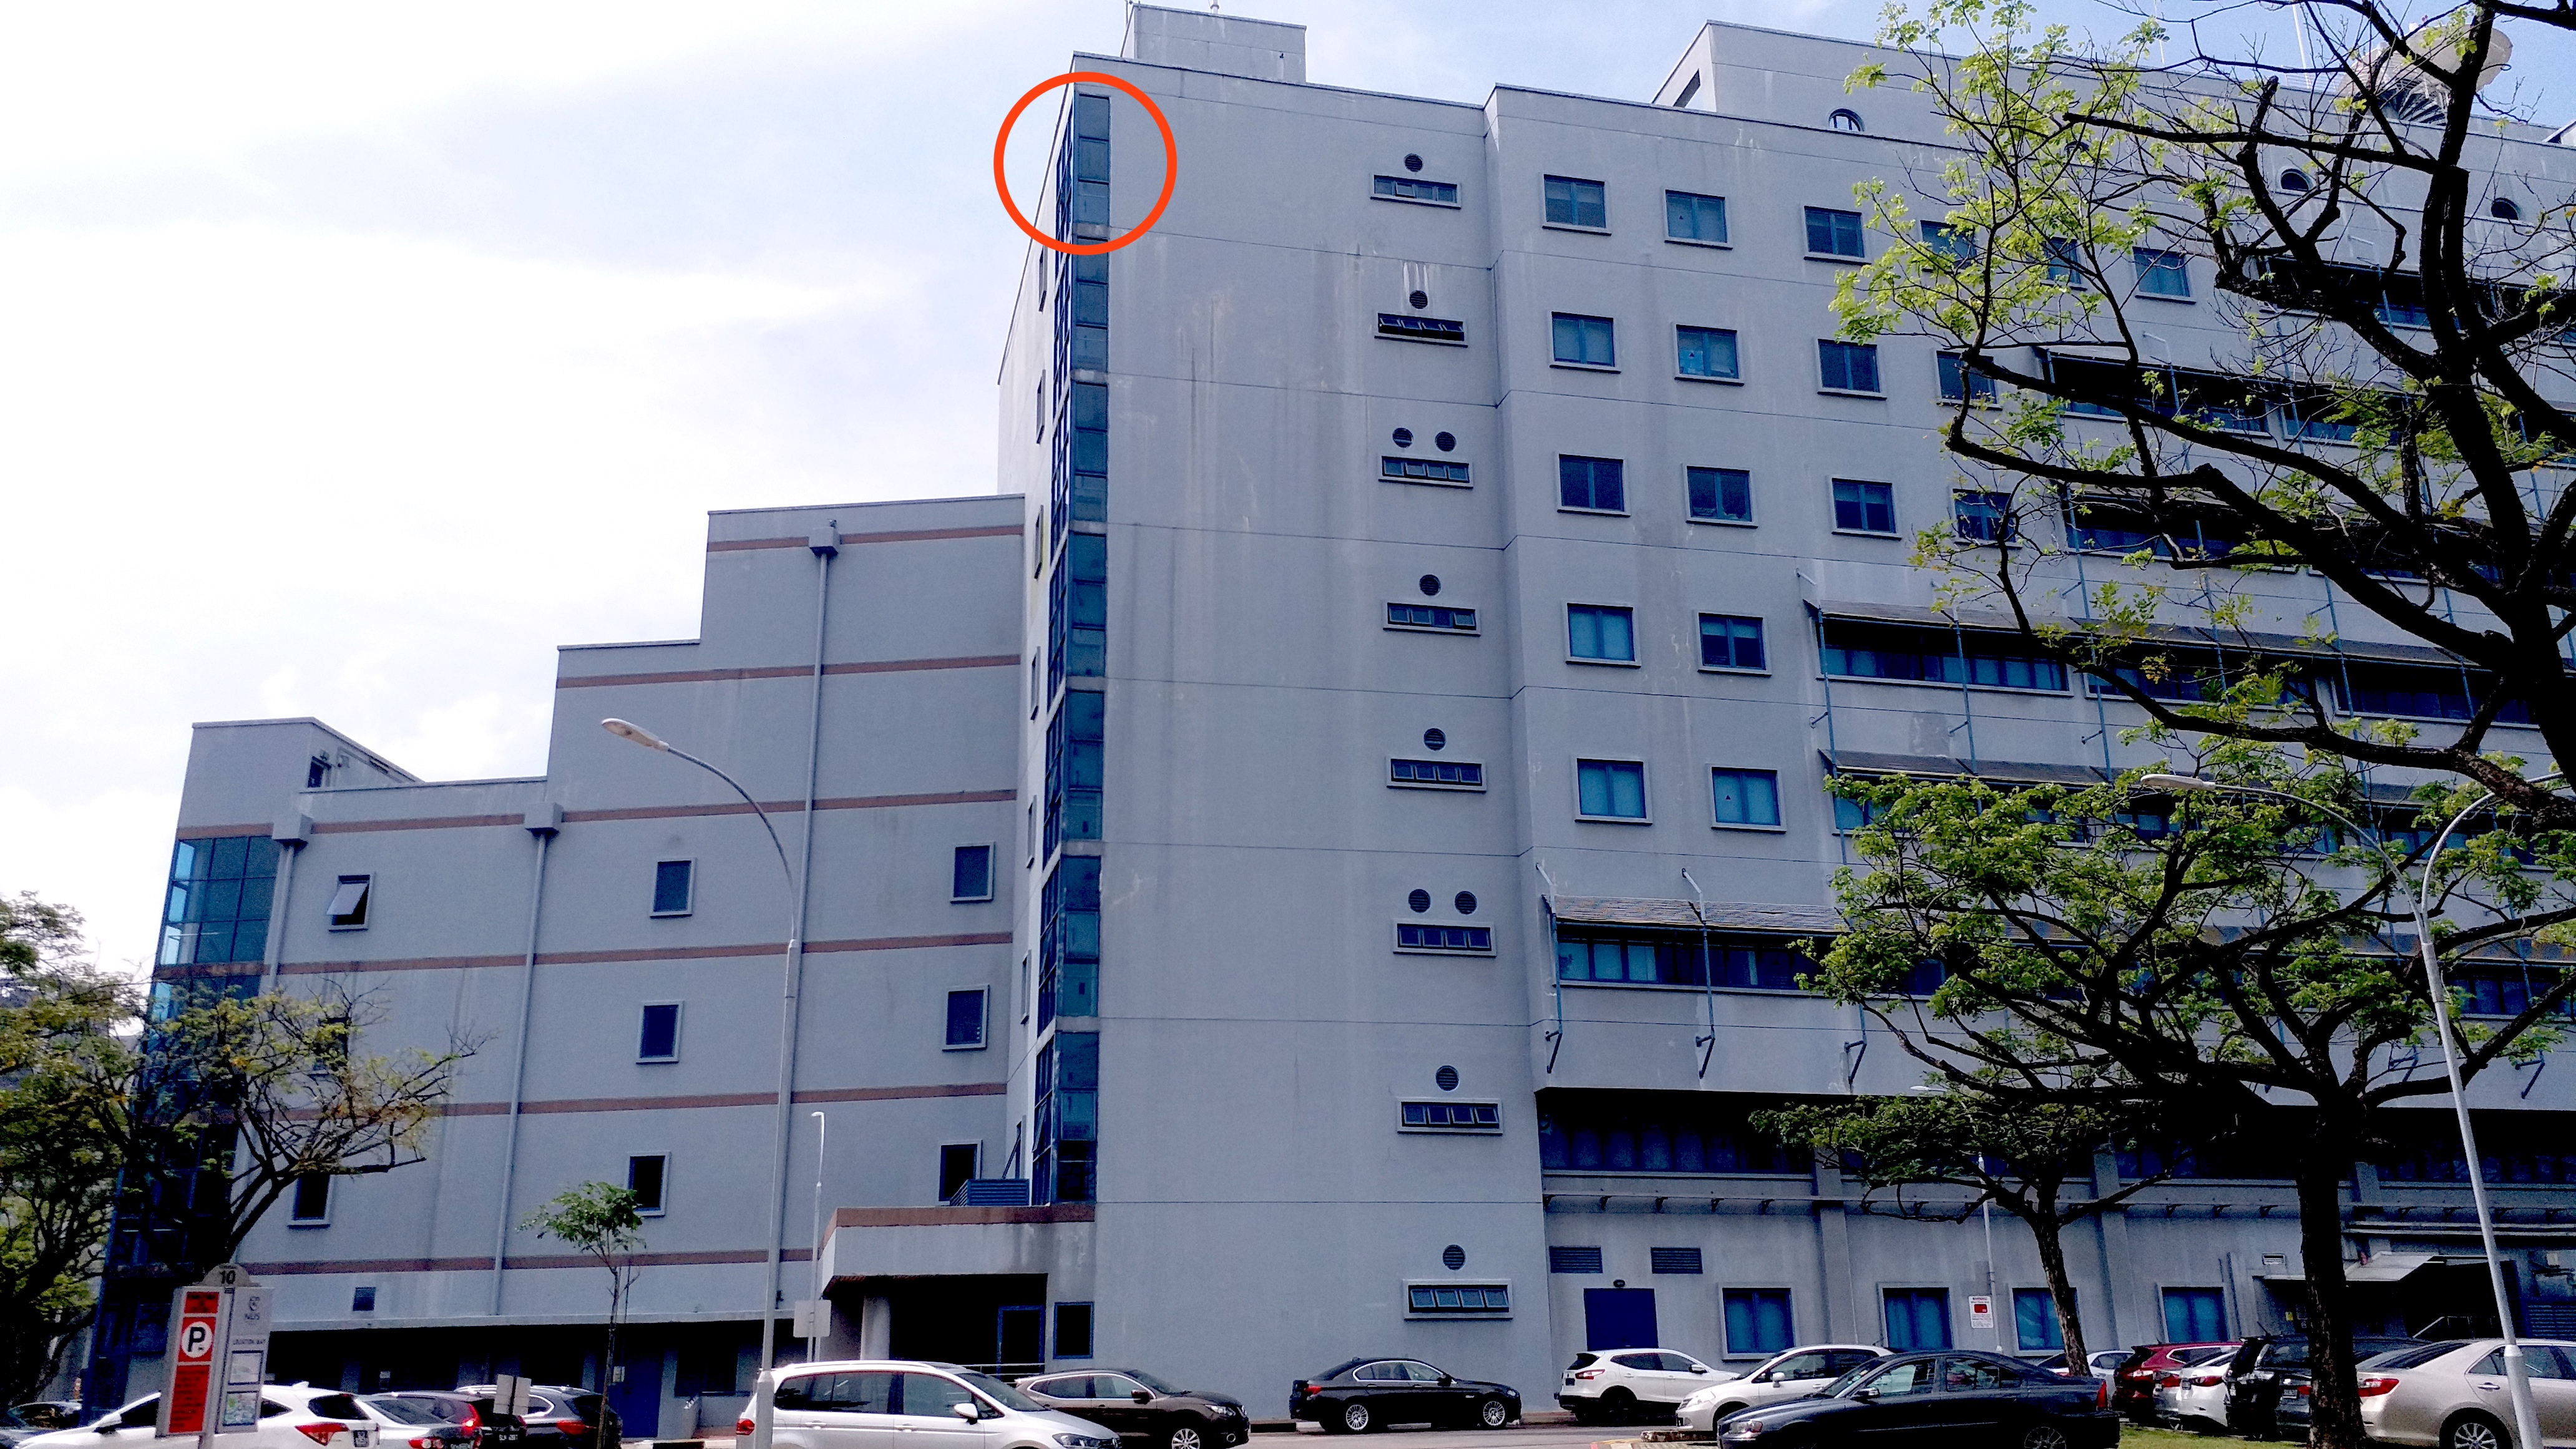
\includegraphics[width=0.5\textwidth]{figures/context_2.jpg}
			\caption{located at the encircled position,}
			\vskip 5mm
			\includegraphics[width=0.5\textwidth]{figures/spots_wo_labels.png}
			\caption{facing the following parking lot.}
		\end{figure}
		\vskip -5mm
		Pictures were taken every five minutes by a Raspberry Pi-based camera, as pictured below:
		\vskip 5mm
		\begin{figure}[H]
			\centering
			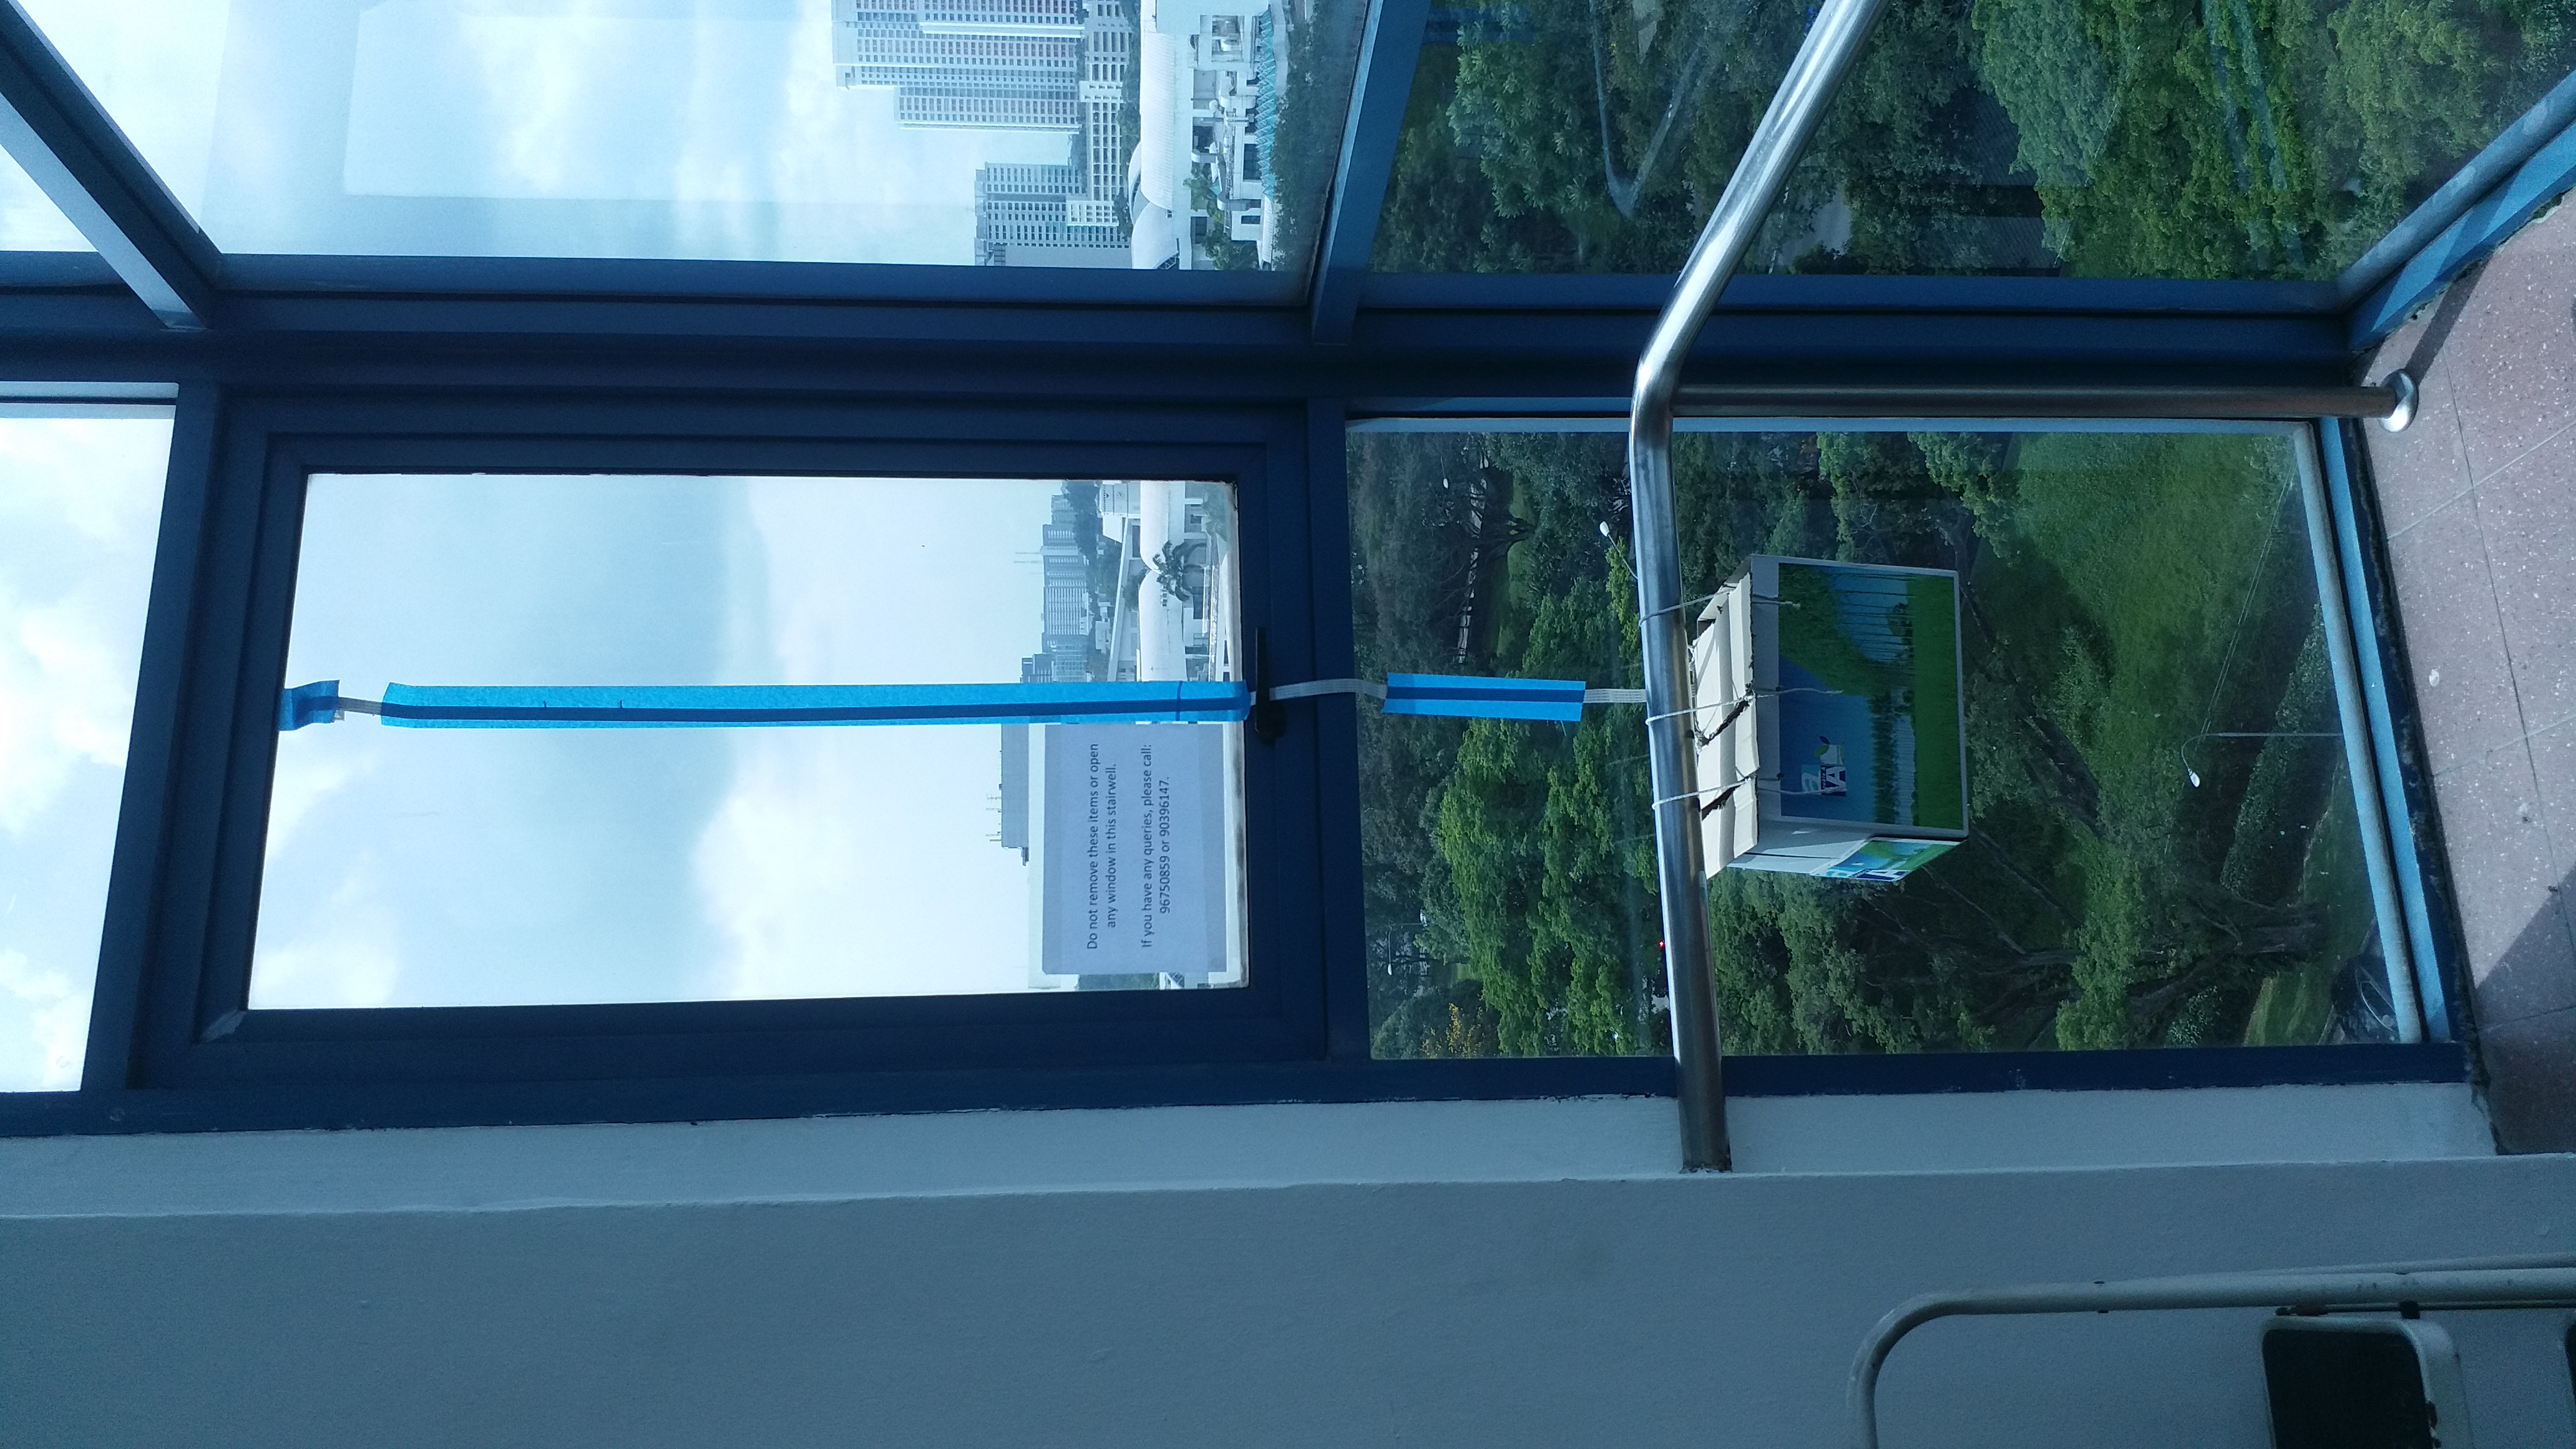
\includegraphics[width=0.4\textwidth]{figures/rpi_camera_1.png}
			\caption{The Raspberry Pi and its memory and power supply were 
			enclosed in the cooled box.}
			\vskip 5mm
			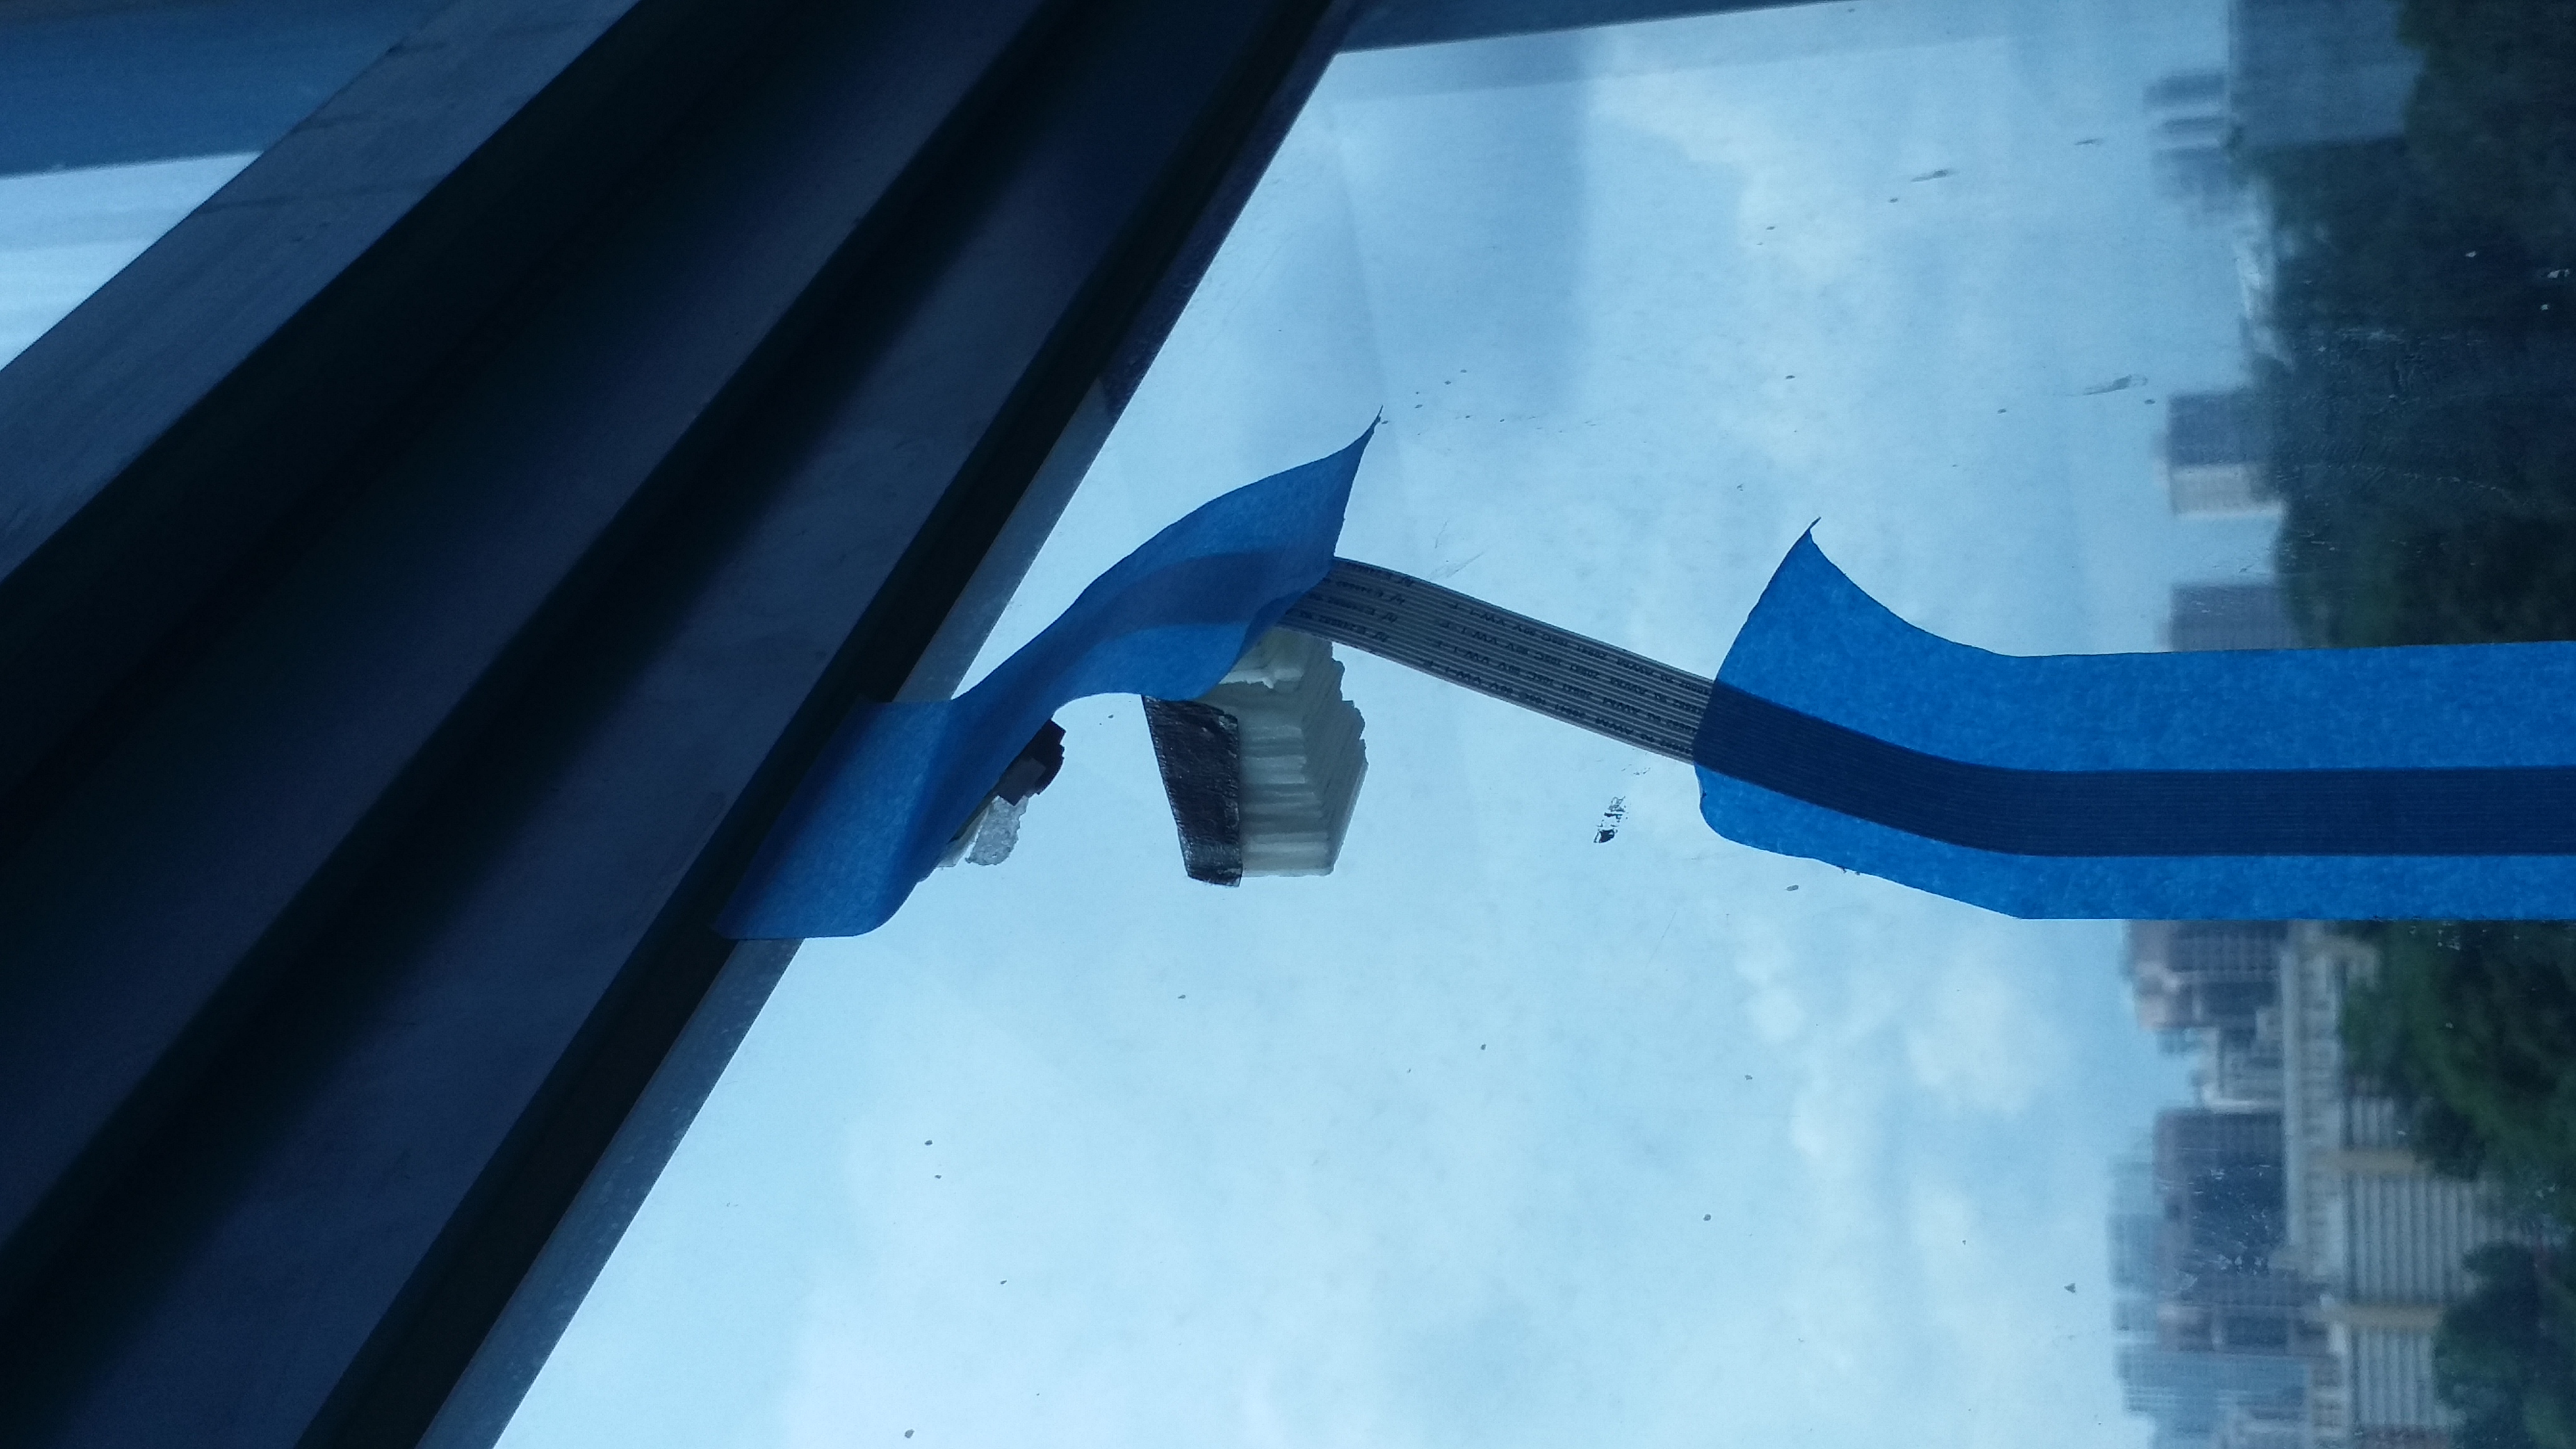
\includegraphics[width=0.4\textwidth]{figures/rpi_camera_2.png}
			\caption{The camera module was mounted firmly on the window at a 
			suitable angle.}
		\end{figure}
		The following is a list of the complete apparatus used:
		\begin{enumerate}
			\setlength\itemsep{-3mm}
			\item Raspberry Pi Model B+, running Raspbian 4.14.
			\begin{itemize}
				\item[] Power supply: 20000 mAh USB powerbank, enclosed in a LiPo battery blast protector.
				\item[] Memory: External 64 GB USB drive.
			\end{itemize}
			\item Raspberry Pi Camera Module V1.
			\begin{itemize}
				\item[] Connected to the Raspberry Pi using a two-meter flex cable.
			\end{itemize}
			\item Portable fan, modified to run off of a USB powerbank.
			\begin{enumerate}
				\item[] Power supply: 10000 mAh powerbank, enclosed in a LiPo battery blast protector.
			\end{enumerate}
		\end{enumerate}
		The powerbanks lasted about a day given the high temperatures at the vantage. The Raspberry Pi 
		and powerbanks were thus removed from the vantage each evening and replaced the subsequent 
		morning. This was also done for security purposes, although the people and license plates were not 
		identifiable in the taken pictures.
	
	\subsection{Cropping of spots from complete images}
		In the evenings, the pictures were cropped and labeled. The cropping process was 
		fully automated	using the scripts of \texttt{label\_examples/crop\_spots/} 
		following a one-time setup. 
		Namely, each spot in the parking lot was assigned an ID for cropping and file-naming purposes:
		\begin{figure}[H]
			\centering
			\includegraphics[width=0.8\textwidth]{figures/spots_w_labels.png}
			\caption{The spots and their IDs.}
		\end{figure}
		For each spot, ``cropping instructions'' were created using\\
		\texttt{label\_examples/crop\_spots/get\_spot\_coords\_and\_angles.py}. This script accepts as flags
		the path to an image and an angle to rotate the image (counter-clockwise) by. It then displays the
		rotated image and allows users to drag-and-click green bounding boxes over it to ascertain the coordinates
		of the region to crop the image to obtain a picture of the desired spot. It prints the coordinates of drawn
		bounding boxes in the terminal from which the script is called. The following is an example of its use:
		\begin{figure}[H]
			\centering
			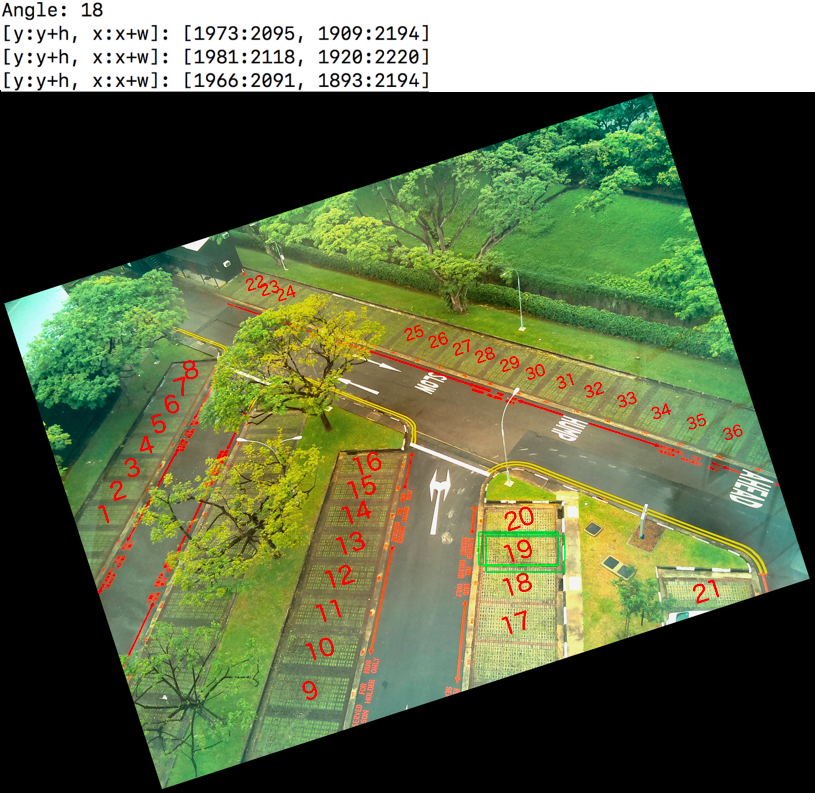
\includegraphics[width=0.75\textwidth]{figures/spot_coord_demo}
			\caption{An example-attempt to obtain the right angle and coordinates to crop images for spot 18.}
		\end{figure}
		This tool was used to get cropping instructions for each spot. These instructions are stored in
		\texttt{label\_examples/crop\_spots/crop\_instructions.csv}. They are 
		accessed by
		\texttt{label\_examples/crop\_spots/crop\_all\_spots.py}, which is itself called by
		\texttt{label\_examples/crop\_spots/daily\_cropper.sh}. The latter is what the user has to call to automatically
		crop all images placed in \texttt{label\_examples/pictures\_dump} into \texttt{label\_examples/pictures\_dump/cropped}.
		The following is thus the cropping workflow:
		\begin{enumerate}
			\item User places all images to be cropped in \texttt{label\_examples/pictures\_dump}, and calls
			\texttt{label\_examples/crop\_spots/daily\_cropper.sh}. 
			\item The script calls \texttt{label\_examples/crop\_spots/crop\_all\_spots.py}, which pipes
			shell commands to obtain the cropped image of each spot from each image to be cropped to
			\texttt{label\_examples/crop\_spots/todo.sh}. These shell commands are calls to
			\texttt{label\_examples/crop\_spots/crop.py}, which crops and saves a specified spot from a
			single image, given its cropping instructions.
			\item \texttt{label\_examples/crop\_spots/todo.sh} is deleted.
		\end{enumerate}
		Thus, apart from manual determination of each spot's cropping instructions, the user is insulated from
		the otherwise tedious cropping process.
		\begin{figure}[H]
			\centering
			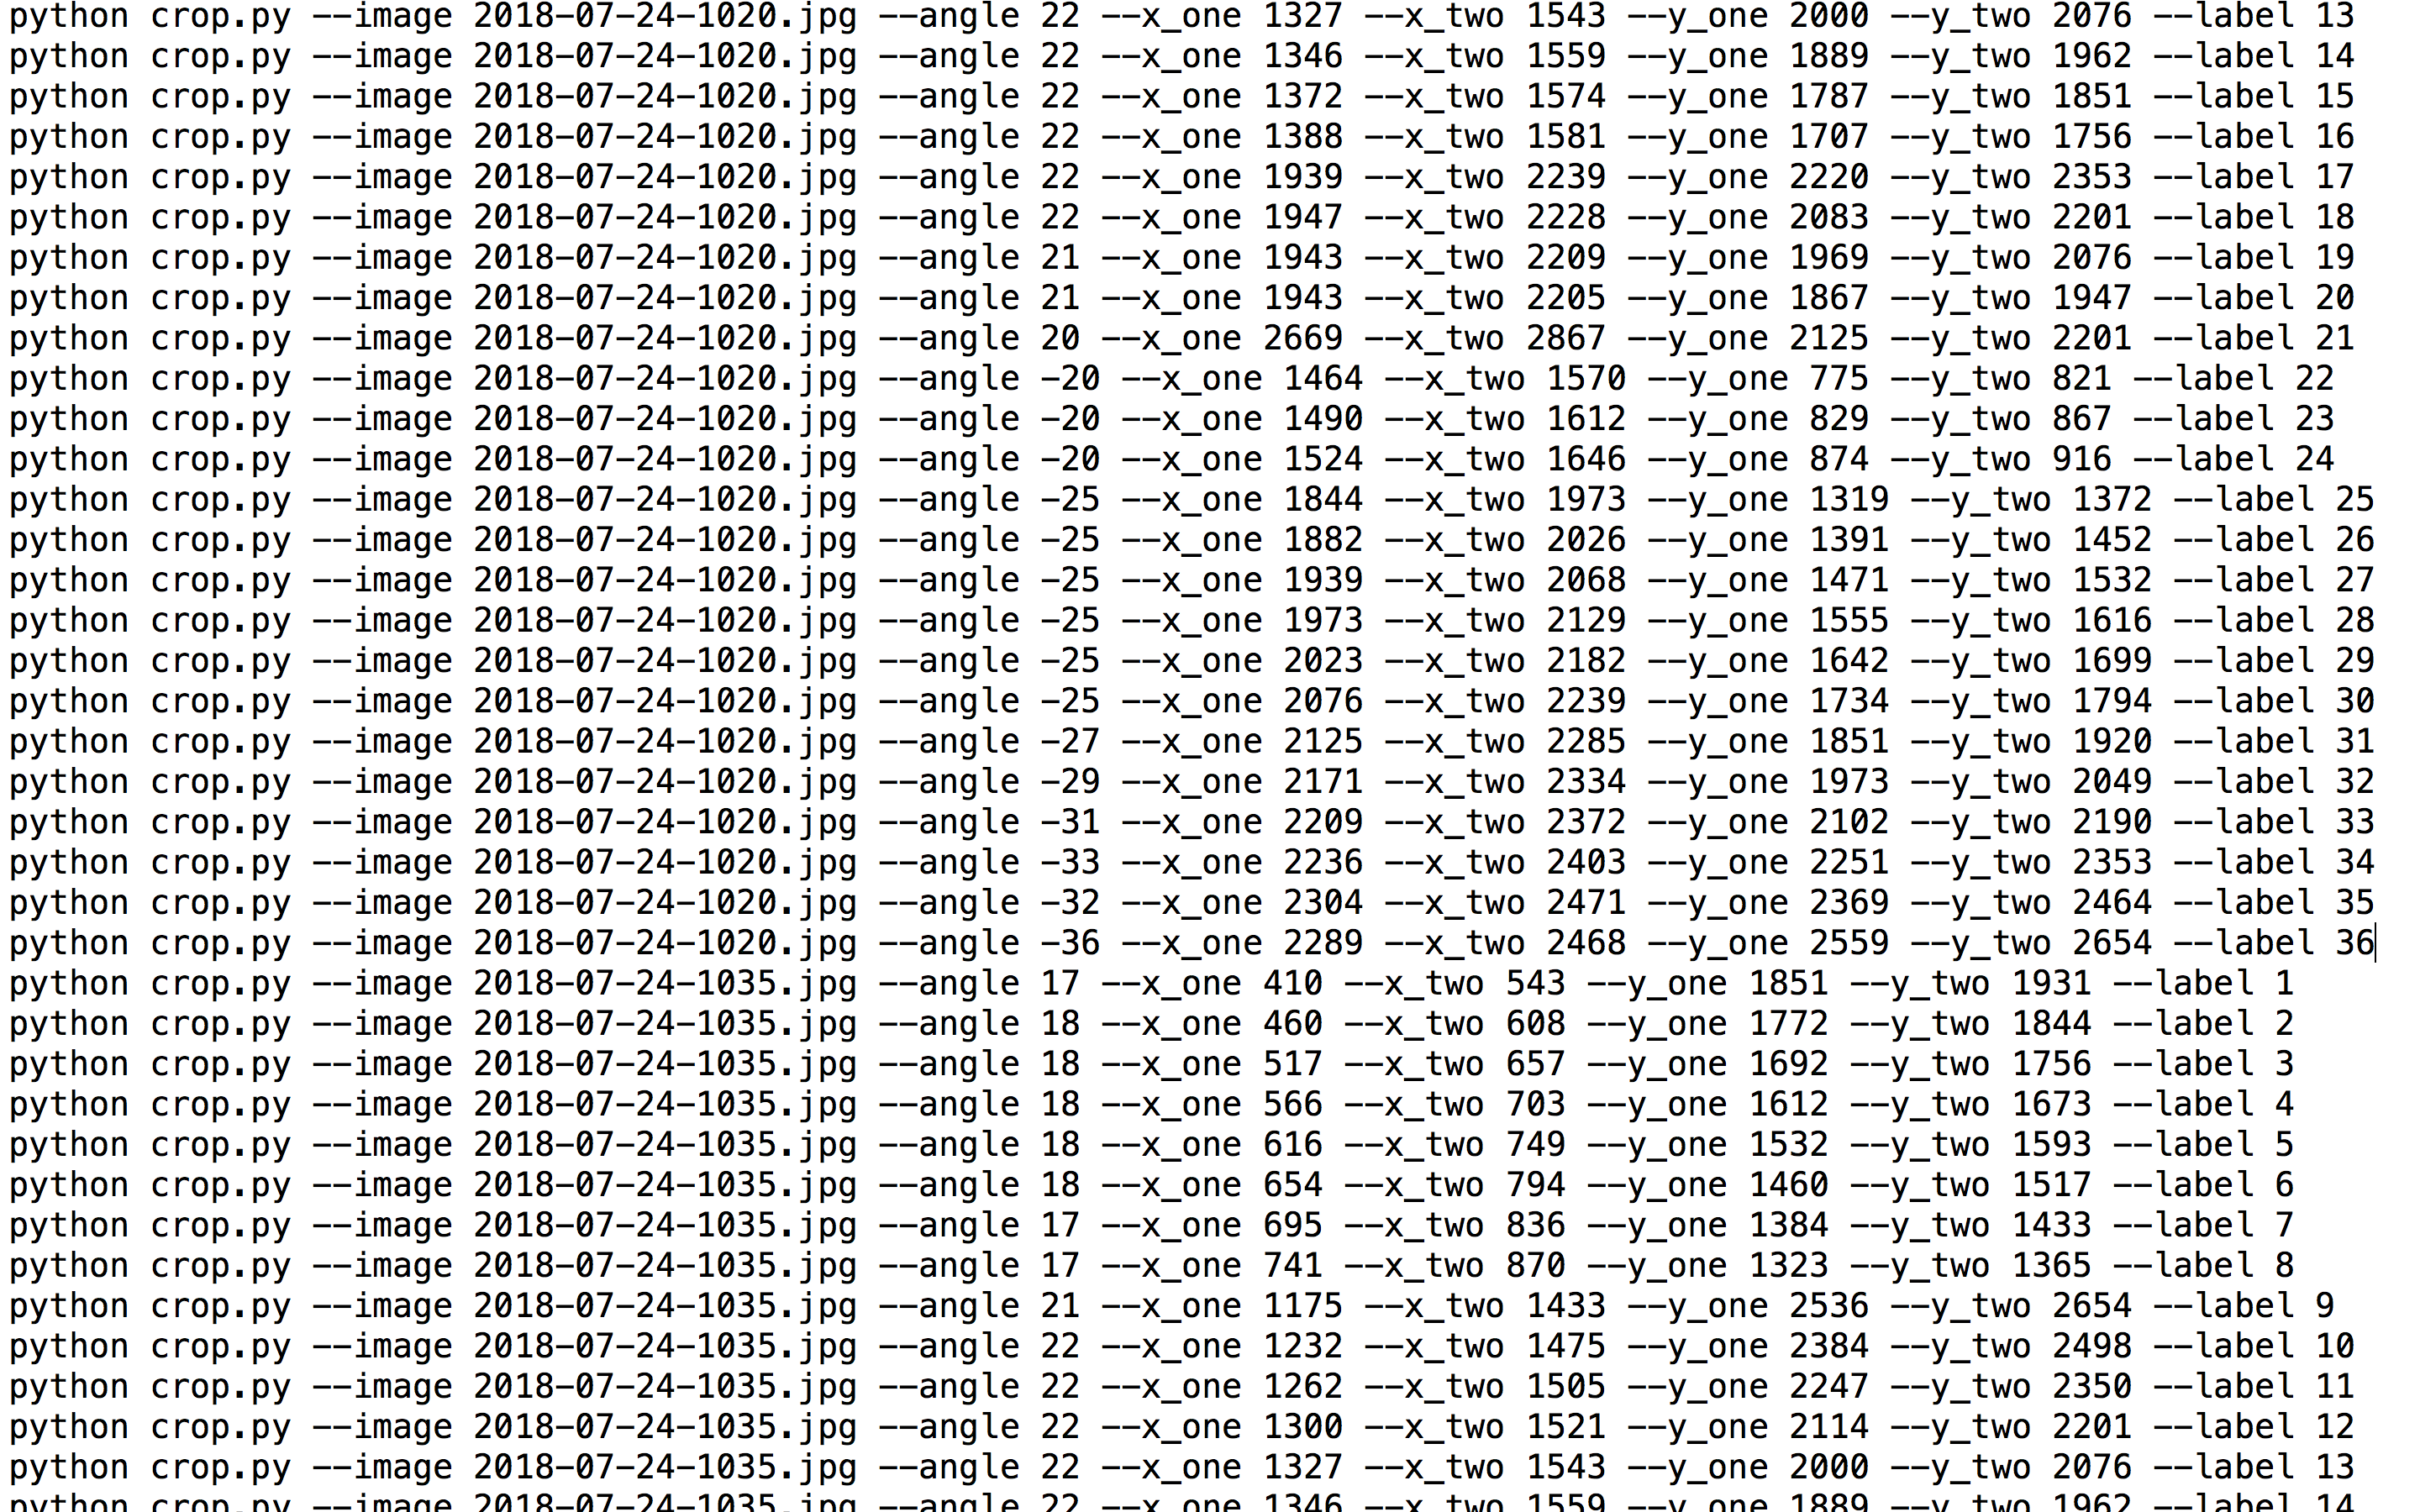
\includegraphics[width=0.8\textwidth]{figures/daily_cropper_example}
			\caption{\texttt{daily\_cropper.sh} generates shell commands to 
			crop all desired images.}
		\end{figure}

	\subsection{Labeling of cropped images}
		After cropping, the resulting images are to be transferred to\\
		\texttt{label\_examples/label\_spots/pictures\_to\_label/} for labeling, 
		which is done using 
		\texttt{label\_examples/label\_spots/spot\_labeler.R}. This script displays
		each cropped image in sequence, prompting the user to type a label for each
		one. In the case of this problem, labels were either ``0'' or ``1'',
		depending on whether the spot was empty or occupied respectively. Once each
		image has been labelled, labels are written to a \texttt{.csv} file
		entitled by the date the images were taken. The following is an example of
		the labeling process:\\
		\begin{figure}[H]
			\centering
			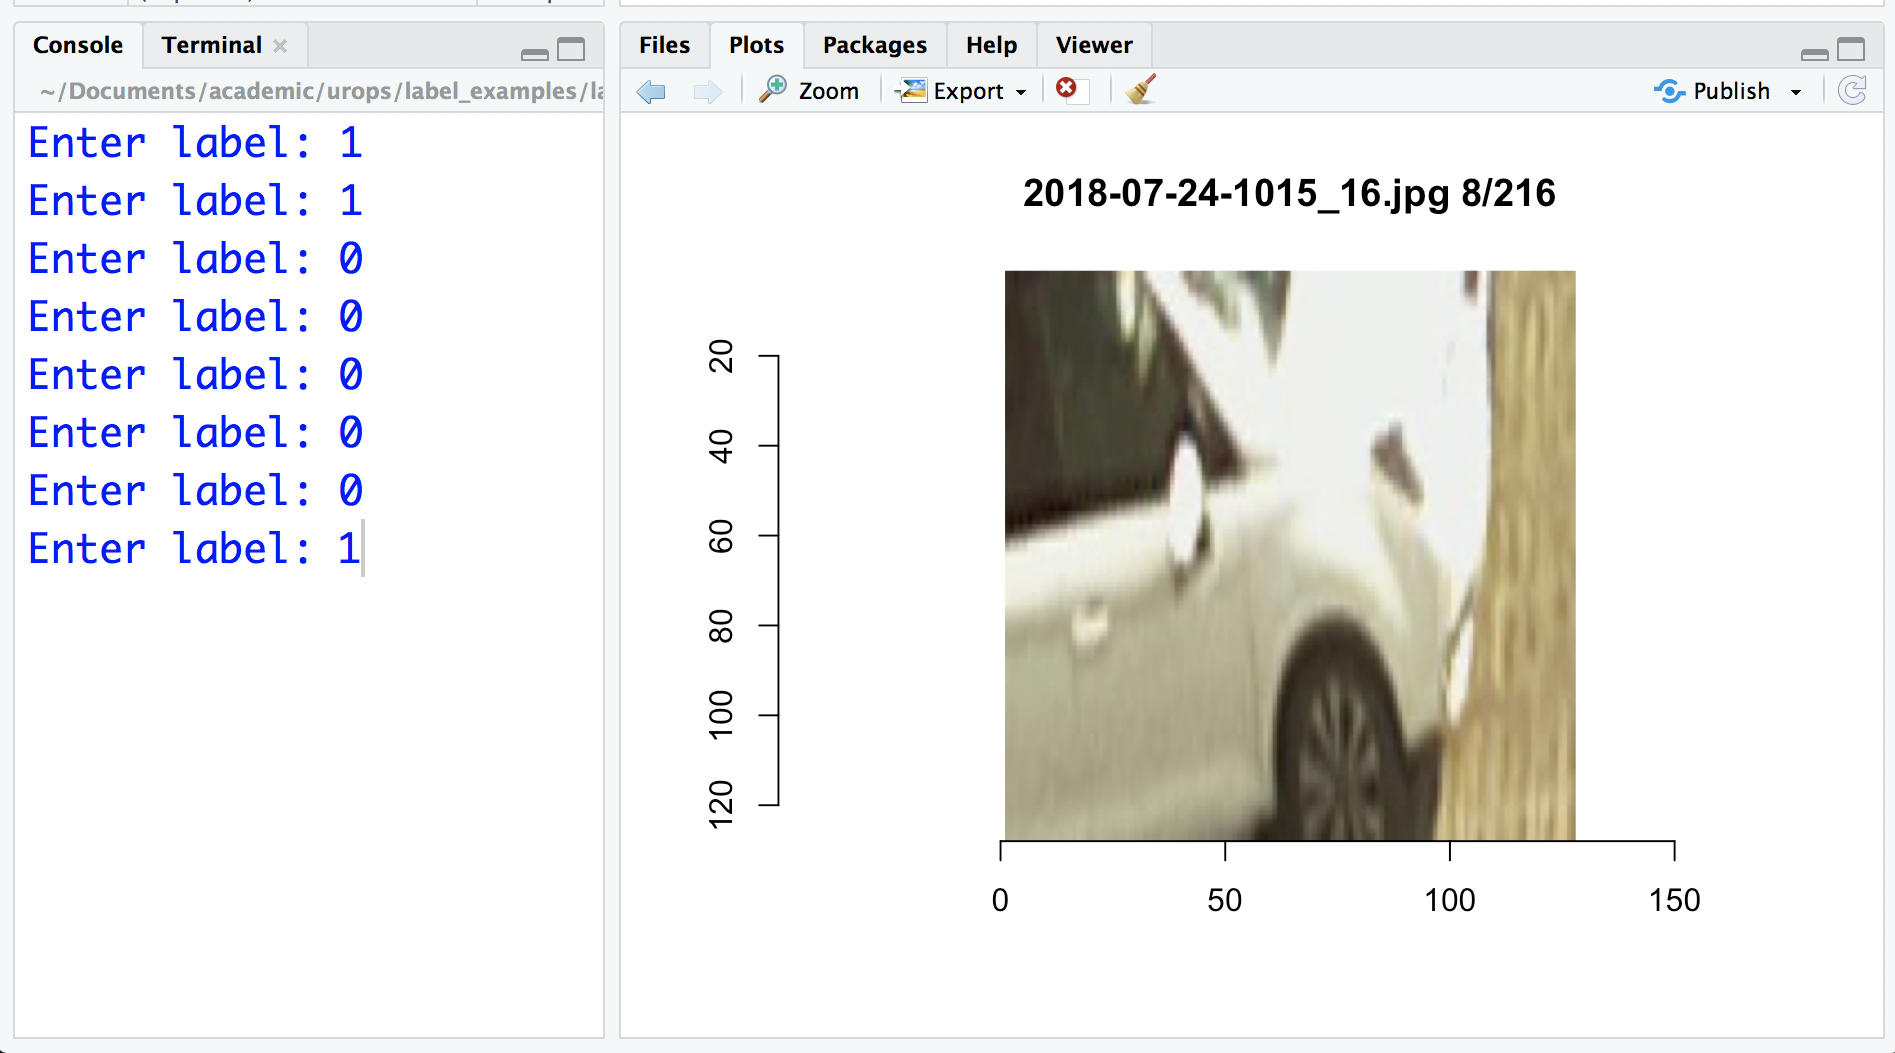
\includegraphics[width=0.8\textwidth]{figures/spot_labeler_example}
			\caption{The image of each spot is displayed in sequence.}
		\end{figure}	
	\subsection{Serialization of data}
		After data collection, processing, and labeling was completed, the data was
		ready to be serialized. Namely, all labels were stored in \texttt{data/labels/} and cropped
		images in \texttt{data/cropped/}, \texttt{save\_dataset/serialize\_dataset.ipynb}
		was used to process the images and labels into NumPy arrays before serialization
		into \texttt{.hdf5} binary files.
		\newpage
		The following is the process:
		\begin{enumerate}
			\item All cropped images and labels are used to create the feature and label matrices
			(respetively).
			\item These matrices are split up randomly into the train and test sets, with the test
			set comprising of 10\% of the total number of examples at hand.
			\item Mean-subtraction and normalization of the test set is 
			conducted using the mean \cite{sub-norm}\relax
			and standard deviation of the training set. The test set is then saved as a
			\texttt{.hdf5} binary file in \texttt{data/hdf5/} as \texttt{test\_set.hdf5}.
			\item The training set matrix is then split into train and validations sets three times,
			to allow for stratified three-fold cross validation. For each split, the train and
			validation sets are mean-subtracted and normalized using the mean of the corresponding
			training set. Each split is then saved
			\texttt{data/hdf5/train\_validation\_set\_{split\_number}.hdf5}, where
			\texttt{split\_number} is one of 1, 2, or 3.
		\end{enumerate}
		Three splits were made instead of the more common five or ten because of memory constraints: each
		split of the training set is 17.7 GB. Given that these scripts may be used to process other data,
		\texttt{save\_data/serialize\_data.ipynb} has been designed to be able to create a variable number
		of splits, and handle a variable number of classes and image types. (In fact, all aforementioned
		scripts can also be applied to the general data-processing context.)
		Also to note is that the third-part \texttt{h5py} module was used to serialize the data into
		\texttt{.hdf5} files instead of the more commonly-used inbuilt \texttt{pickle} module since
		the former module is far more memory-efficient for the serialization of 
		numerical arrays \cite{hdf5-performance}\relax.

	\subsection{Culmination}
		After the completion of the above, the dataset was ready to use for machine learning purposes. It
		has been uploaded to Google Drive as \texttt{NUSLot}
		\hyperlink{https://goo.gl/fV2NXS}{goo.gl/fV2NXS}, and comprises of 
		three sub-directories:
		\begin{enumerate}
			\item \texttt{raw\_data} comprises of ``complete'' parking lot images, cropped images of
			individual spots, and all label \texttt{.csv} files.
			\item \texttt{full\_dataset} comprises of serialized NumPy arrays 
			representing
			training, validation, and testing sets created from all 50,000 examples. 
			\item \texttt{toy\_dataset}, is a 10\% simple random sample of the 
			data of
			\texttt{full\_dataset}.
		\end{enumerate}

\section{Implementation of the CNN}
	The CNN was implemented on Tensorflow version 1.9. It was created using this library's low-level API to
	allow for greater extensibility and functionality, which will be described in this section. Firstly, however,
	a description of the architecture and hyperparameters of the CNN used for this classification problem:
	\begin{itemize}
		\setlength\itemsep{-3mm}
		\item[] (Learning rate: 0.0001)
		\item[] Input layer: reads in 128-by-128 color images of parking spots.
		\item[] Convolutional layer 1: applies 64 5-by-5 filters, and then the 
		scaled exponential linear unit (SeLU) activation function.
		\item[] Dropout is applied with a keep probability of 0.95.
		\item[] Pooling layer 1: performs max pooling with a 2-by-2 filter.
		\item[] Convolutional layer 2: applies 128 3-by-3 filters, and then the 
		SeLU activation function.
		\item[] Dropout is applied with a keep probability of 0.95.
		\item[] Pooling layer 2: performs max pooling with a 2-by-2 filter.
		\item[] Convolutional layer 3: applies 256 3-by-3 filters, and then the 
		SeLU activation function.
		\item[] Dropout is applied with a keep probability of 0.95.
		\item[] Pooling layer 3: performs max pooling with a 2-by-2 filter.
		\item[] Convolutional layer 4: applies 512 3-by-3 filters, and then the 
		SeLU activation function.
		\item[] Dropout is applied with a keep probability of 0.95.
		\item[] Pooling layer 4: performs max pooling with a 2-by-2 filter.
		\item[] Convolutional layer 5: applies 1024 3-by-3 filters, and then 
		the SeLU activation function.
		\item[] Dropout is applied with a keep probability of 0.95.
		\item[] Pooling layer 5: performs max pooling with a 2-by-2 filter.
		\item[] Convolutional layer 6: applies 2048 1-by-1 filters, and then 
		the SeLU activation function.
		\item[] Dropout is applied with a keep probability of 0.95.
		\item[] Pooling layer 6: performs max pooling with a 2-by-2 filter.
		\item[] Fully-connected layer 1: comprises of 2048 neurons.
		\item[] Dropout is applied with a keep probability of 0.90.
		\item[] Output layer: 2 neurons, representing the output vector.
		\vspace*{-4mm}
		\begin{enumerate}
			\setlength\itemsep{-3mm}
			\item[] (0, 1) $\rightarrow$ occupied spot
			\item[] (1, 0) $\rightarrow$ empty spot
		\end{enumerate}
	\end{itemize}
	This network, trained over 20 epochs, has a testing accuracy of 99.9\%, a specificity of about 1, and a
	sensitivity of 0.998. As found in ST2288, CNNs are effective for this 
	binary classification task. talk about actual numbers then talk about 
	occlusion -- use the confusion matrix.
	Actually, bring up the occlusion problem here, and talk about specificity 
	so good that occlusion was not an issue, and show a picture of an occluded 
	spot here.
	\begin{figure}
		\centering
		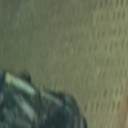
\includegraphics[width=2cm]{figures/nuslot_occlusion}
		\caption{One of the many instances of occlusion that it was not 
		bothered by}
	\end{figure}

	What is more significant is the implementation of this CNN is its 
	extensibility; most readily-available implementations of CNNs tend to not 
	be so \footnote{Consider the canonical
	\hyperlink{https://github.com/aymericdamien/TensorFlow-Examples}
	{github.com/aymericdamien/TensorFlow-Examples} and 
	\hyperlink{https://www.tensorflow.org/versions/r1.0/get\_started/mnist/pros}
	{tensorflow.org/versions/r1.0/get\_started/mnist/pros}}:
	\begin{enumerate}
		\item Automatic data management:
		\item Dynamic scaling of network depth:
		\item Ability to write evaluation mistakes to disk: 
		entitled\_24\_t-1\_p-0
		\begin{figure}[H]
			\centering
			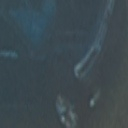
\includegraphics[width=2cm]{figures/mistake_example}
			\caption{lalala}
		\end{figure}
		\item Seamless model saving and restoration options:
		\item Dropout more options: \cite{dropout}\relax 
	\end{enumerate}
	Apart from these more novel features, it also contains the following 
	functionality:
	\begin{enumerate}
		\item Integration with Tensorboard, a visualization suite for 
		Tensorflow: Tensorboard dynamically shows things. Also say you can 
		control summary frequency.
		\begin{figure}[H]
			\centering
			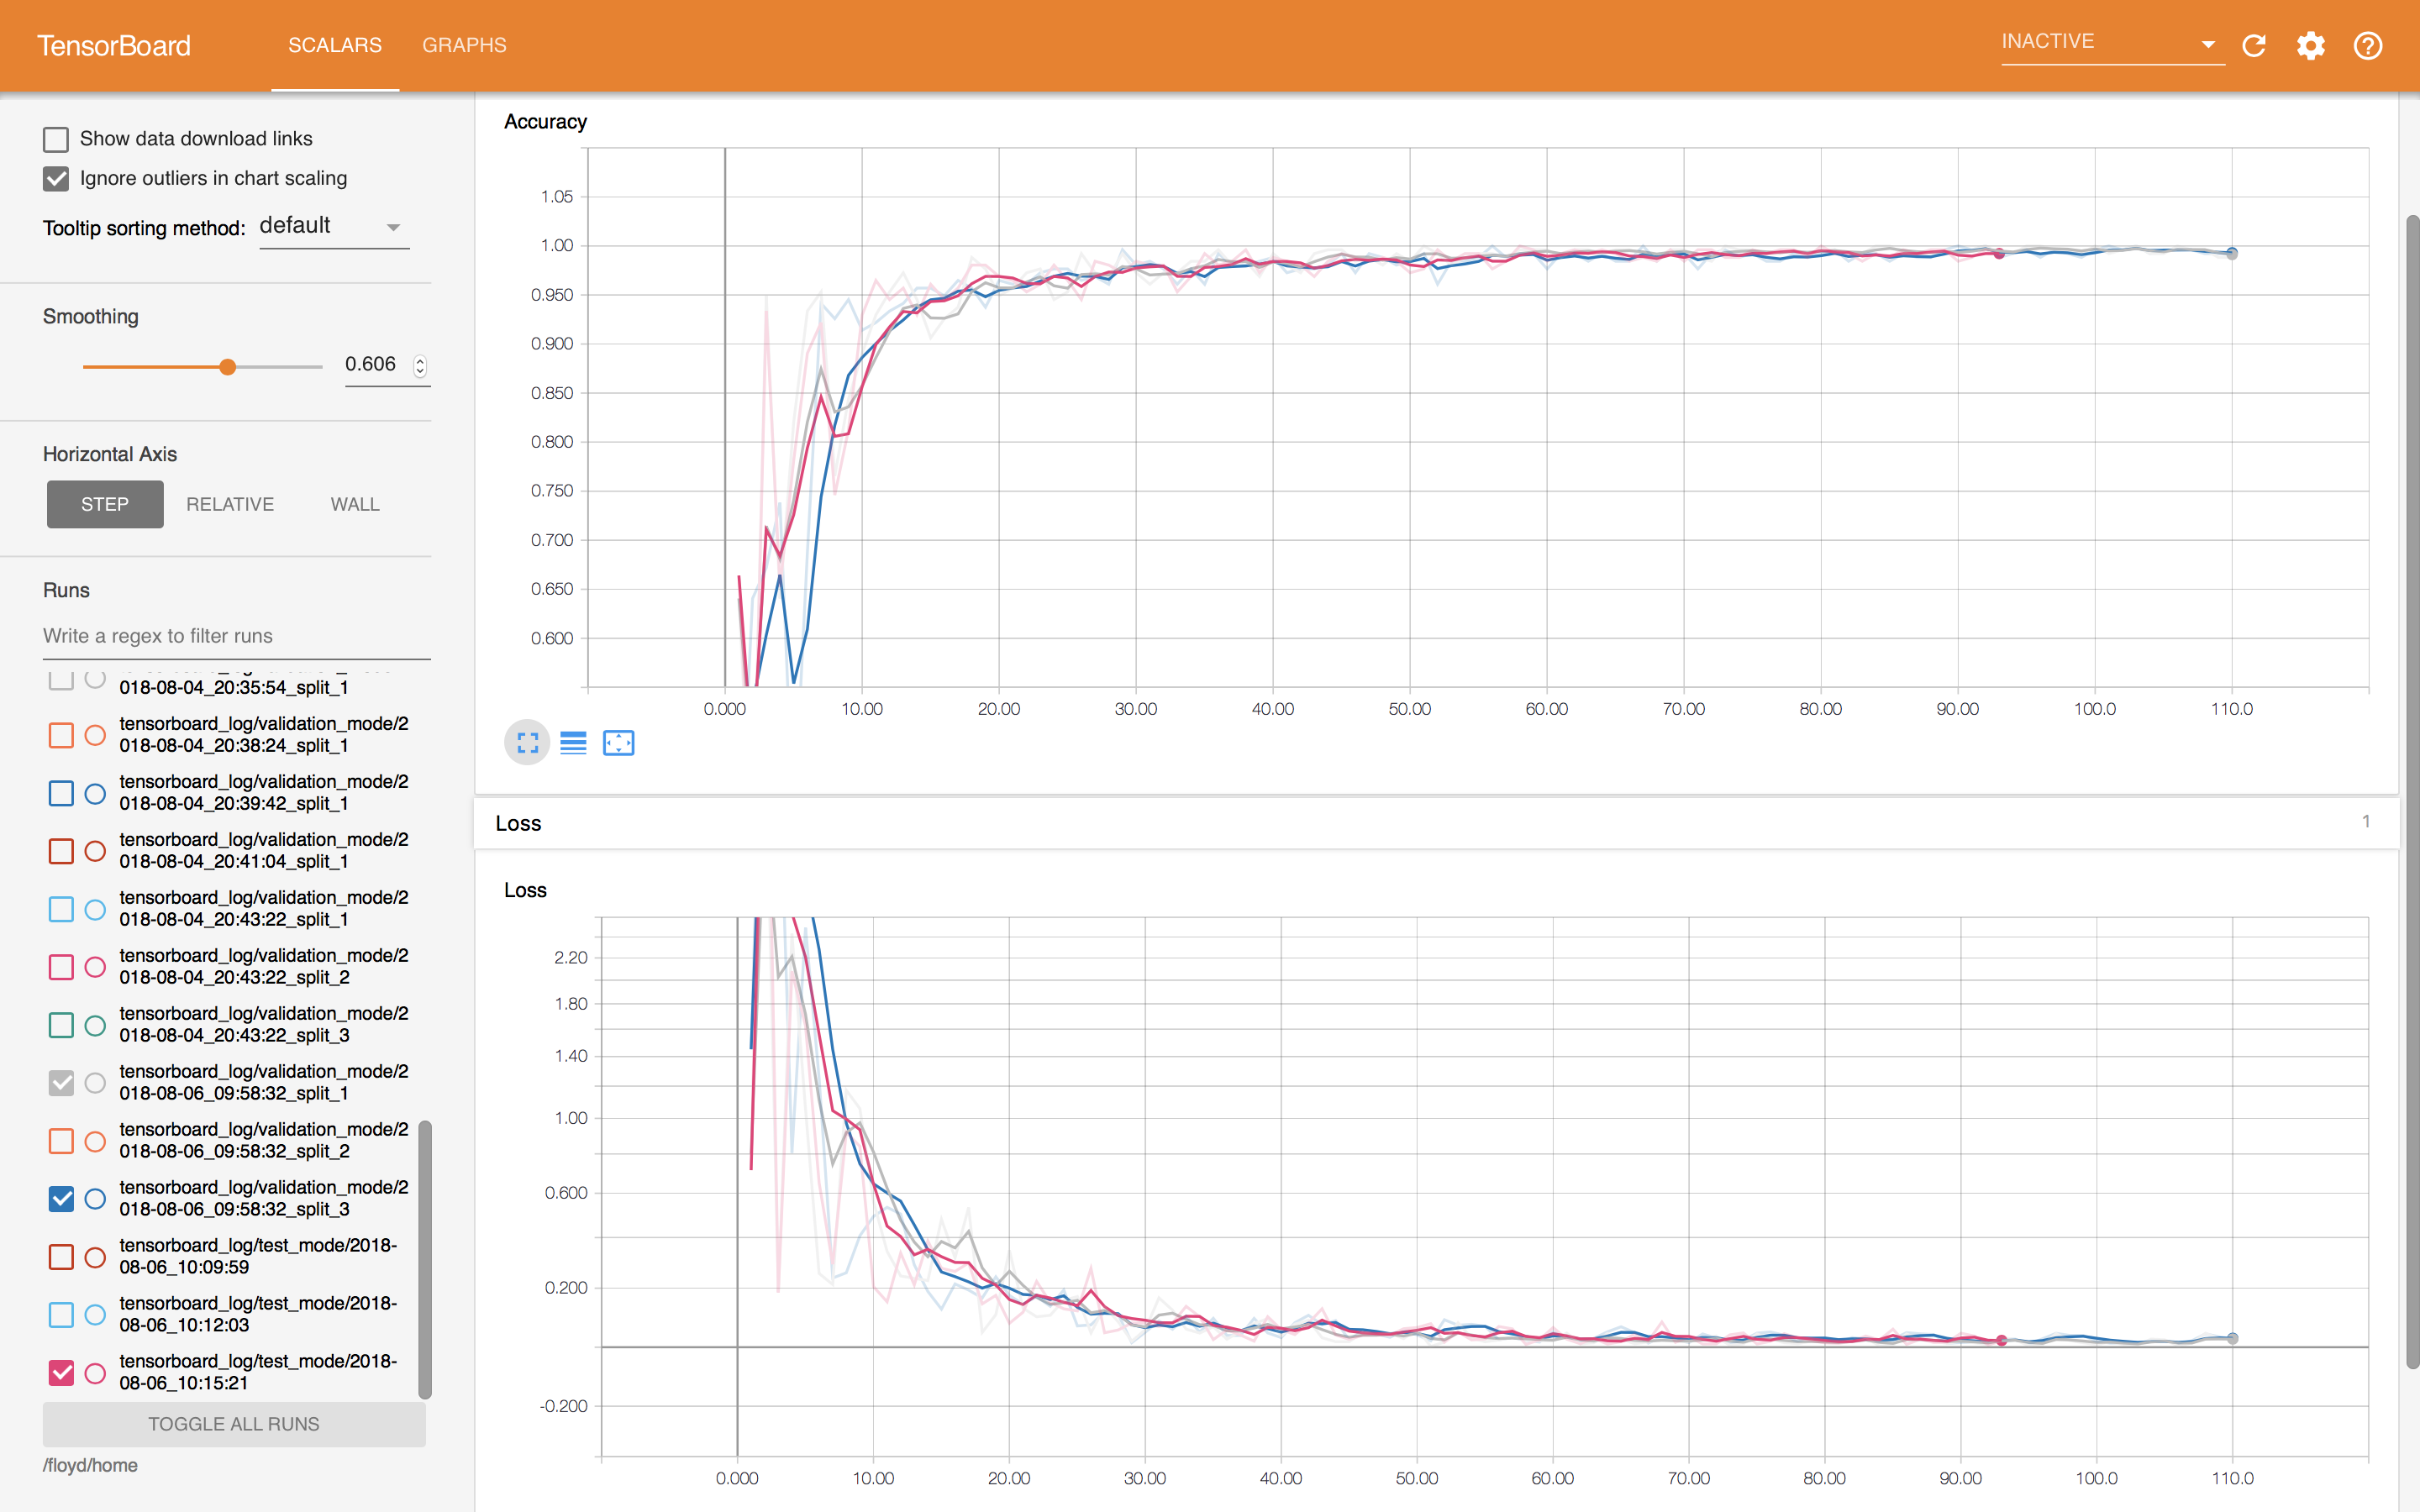
\includegraphics[height=3cm]{figures/tb_acc_loss}
			\caption{lalala}
		\end{figure}
		\begin{figure}[H]
			\centering
			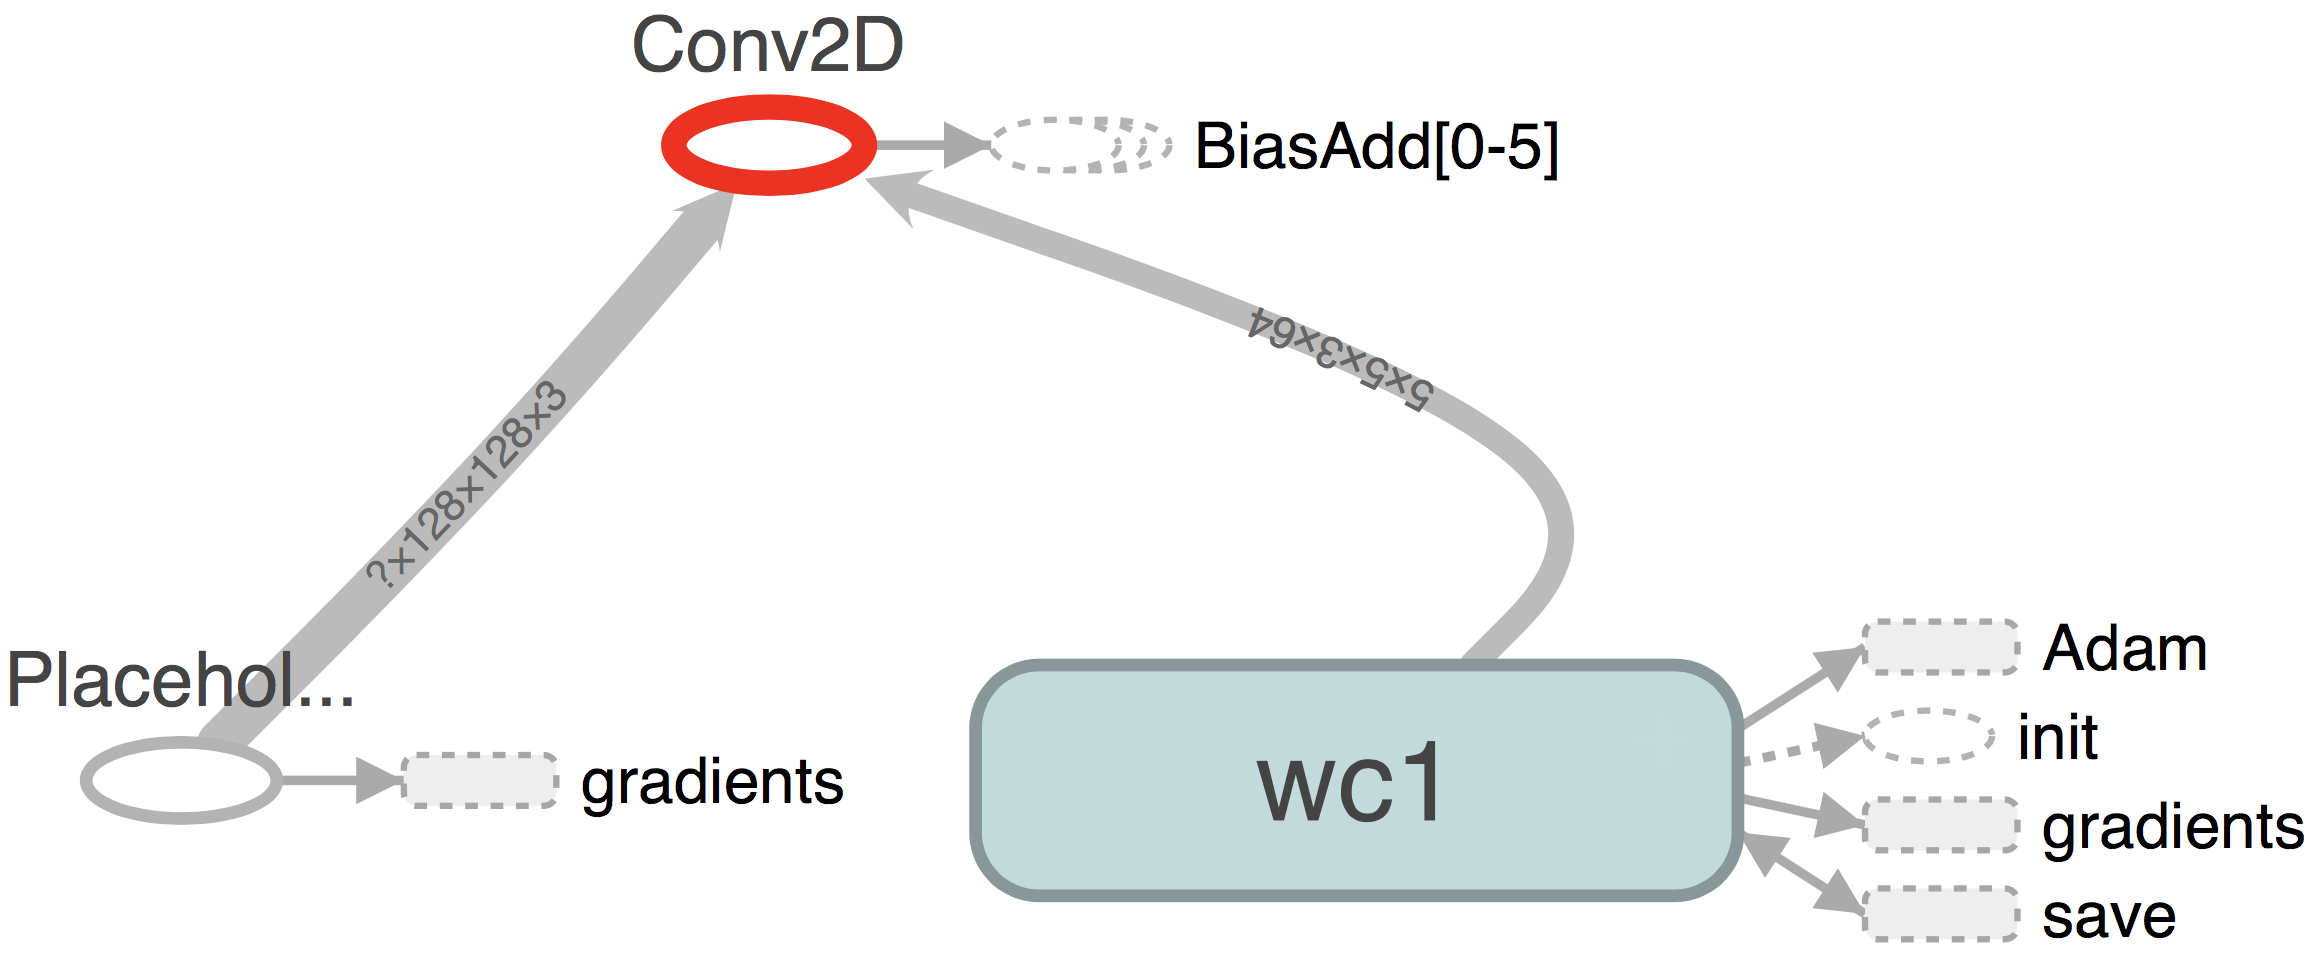
\includegraphics[height=5cm]{figures/tb_graph_2}
			\caption{lalala}
		\end{figure}
		\begin{figure}[H]
			\centering
			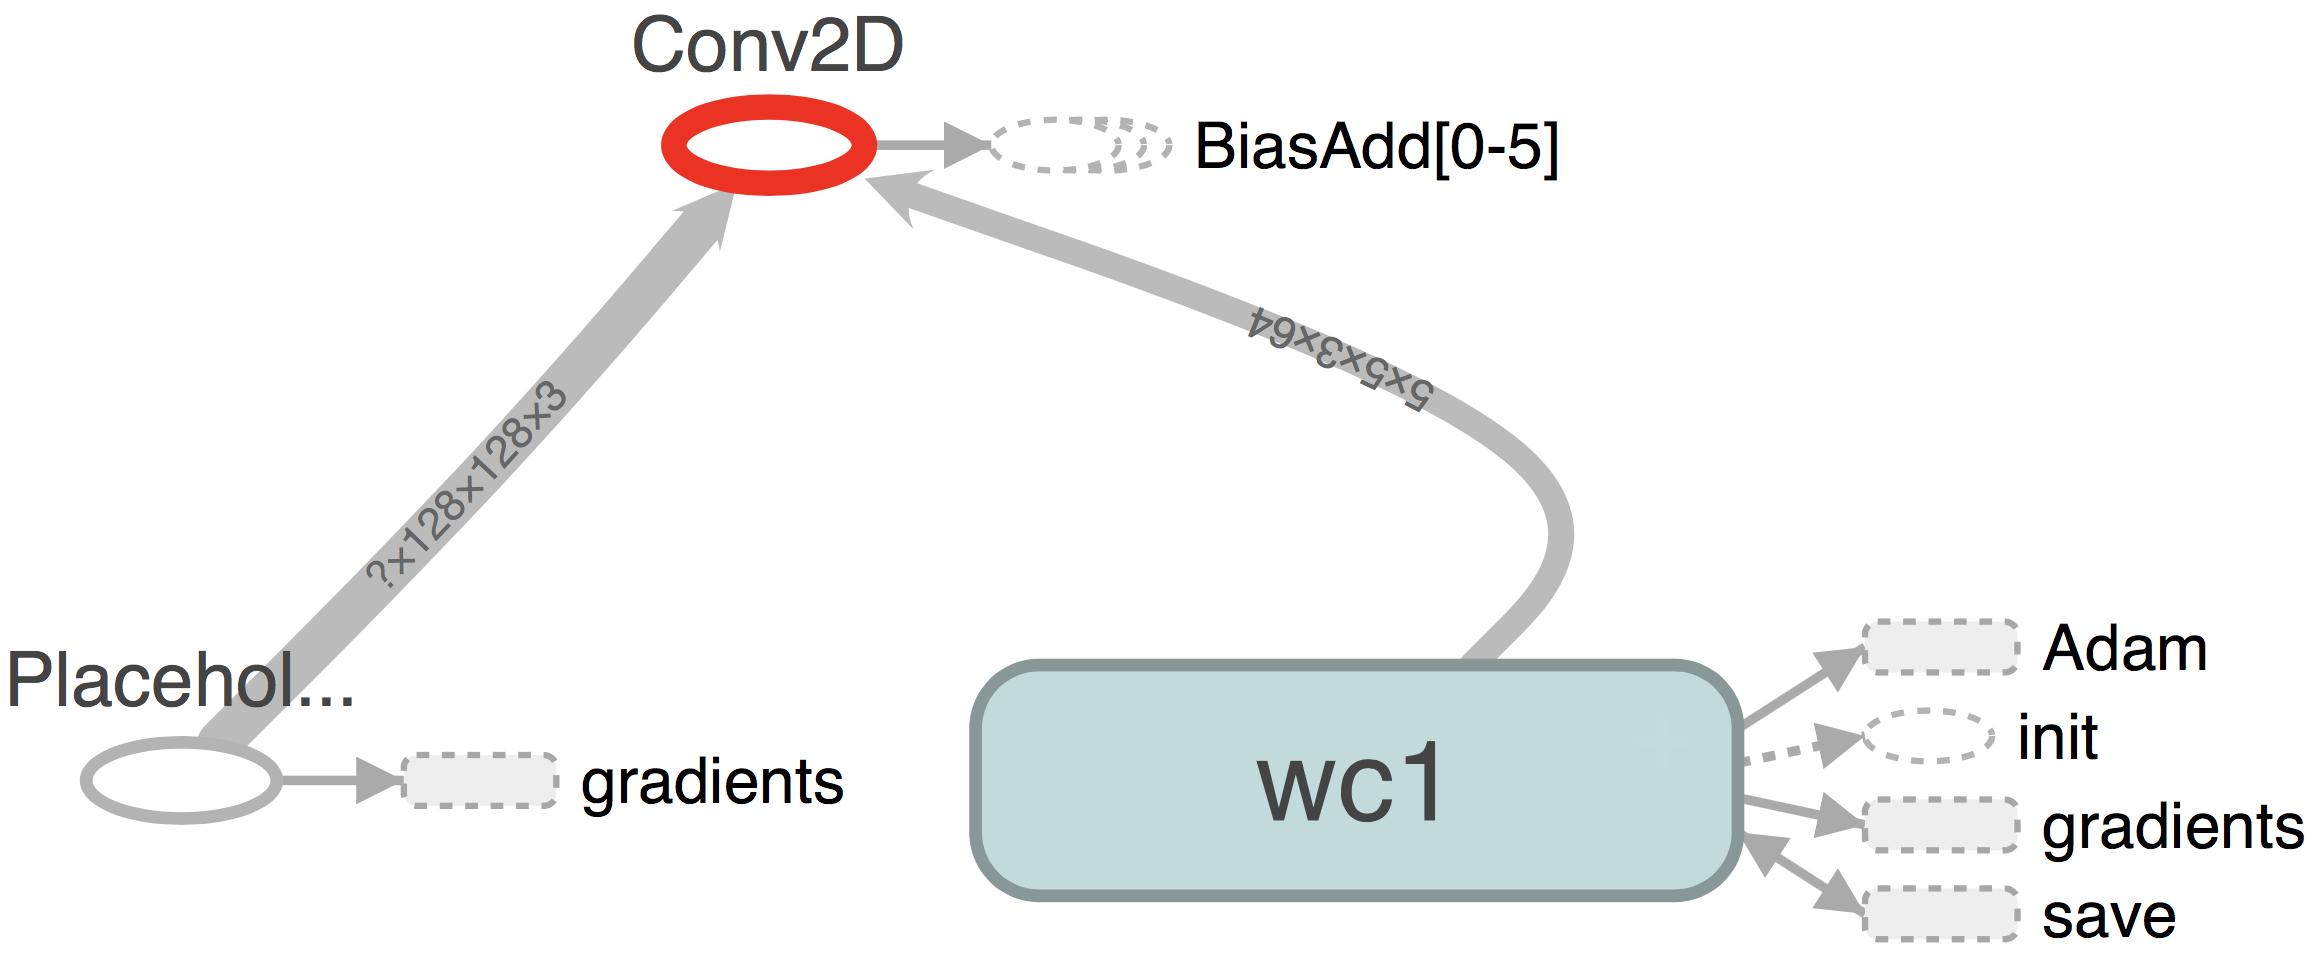
\includegraphics[height=5cm]{figures/tb_graph_1}
			\caption{lalala}
		\end{figure}
		\item End-user encapsulation from adjustment of hyperparameters, 
		activation function and choices: \cite{selu-motivation} \footnote{See 
		\hyperlink{https://github.com/shaohua0116/Activation-Visualization-Histogram}
			{github.com/shaohua0116/Activation-Visualization-Histogram}}
		\item Enhanced evaluation metrics:
		\begin{figure}[H]
			\centering
			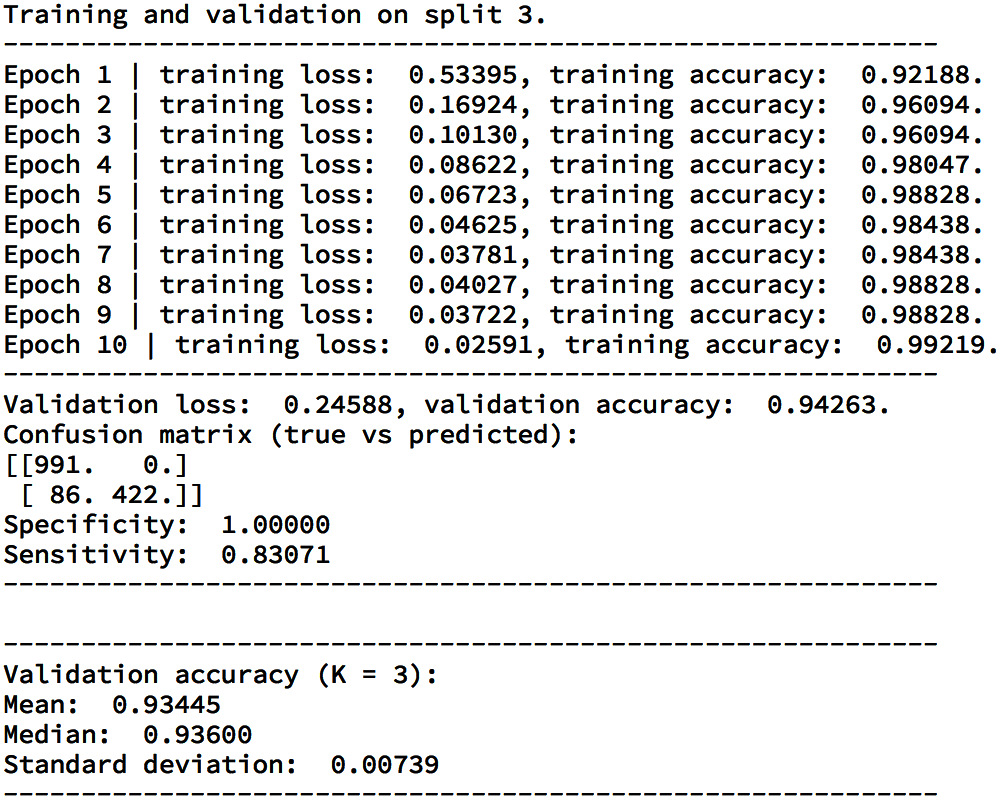
\includegraphics[height=5cm]{figures/floydhub_results_example}
			\caption{lalala}
		\end{figure}
	\end{enumerate}
	Thus, this user-friendly implementation of a CNN on Tensorflow is yet 
	another 

\section{Conclusion}
	This project was carried out with the intention to explore the practicality 
	and effectiveness of the use of CNNs to ascertain the occupancy status a 
	parking lot given pictures of it. Fortunately, performance on both an 
	external and locally-sourced dataset was extremely good. However, and 
	surprisingly, there are significant practical challenges to the setting-up 
	of picture-taking hardware. Some of 
	
	the intricacies and challenged involved in the process of 



	Tell them your honest criticisms of it here, and how you learned that things
	might not be suitable.
	Also talk about how there is a standard way to learn about this stuff, but
	not a standard way to go from learning to implementation, and that given your
	experiences you hope that while what was found here was not ground breaking,
	there is significant merit to this extensible thing and say exactly how it is
	extensible.

	The approach to the second objective, creation of the mobile application, is
	dependent on the experiences from the first. Namely, the second objective will
	require upgrade of the camera to one that is Internet-connected; powering and
	reliably connecting such a device can be challenging.  Moreover, the CNN will
	need to be placed on the cloud, with a suitable interface to handle
	communication between the camera(s) taking the picture upon user request, the
	 model serving the prediction, and the user's mobile application.
	  Nonetheless, increasing the
	resolution of information available to those seeking a parking spot is not the
	only implication of this project, especially given that NUS' parking lots are
	organized appropriately for demand. Rather, we truly view this project as a
	capability-building exercise; a segue into greater problems that can be
	addressed by machine learning--either by us or those who take reference to our
	experiences in the future.

\newpage
\begin{thebibliography}{unsrt}
	\bibitem{pklot-paper}
		Almeida, P. R., Oliveira, L. S., Britto, A. S., Silva, E. J., \& Koerich, A. L. (2015). PKLot--A robust 
		dataset for parking lot classification. \textit{Expert Systems with Applications}, 42(11), 
		4937-4949. doi:10.1016/j.eswa.2015.02.009
	\bibitem{hdf5-performance}
		Finch, C. (2010, January 10). Storing large Numpy arrays on disk: 
		Python Pickle vs. HDF5 [Web log post]. Retrieved August 6, 2018, from 
		https://shocksolution.com/2010/01/10/storing-large-numpy-arrays-on-disk-python-pickle-vs-hdf5adsf/
	\bibitem{sub-norm}
		CS231n Convolutional Neural Networks for Visual Recognition: Setting up 
		the data and the model. (n.d.). Retrieved August 6, 2018, from 
		http://cs231n.github.io/neural-networks-2/
	\bibitem{selu-motivation}
		Pedamonti, D. (2018). Comparison of non-linear activation functions for 
		deep neural networks on MNIST classification task. Retrieved August 6, 
		2018, from https://arxiv.org/abs/1804.02763v1 arXiv:1804.02763v1
	\bibitem{dropout}
		Srivastava, Nitish \& Hinton, Geoffrey \& Krizhevsky, Alex \& 
		Sutskever, Ilya \& Salakhutdinov, Ruslan. (2014). Dropout: A Simple Way 
		to Prevent Neural Networks from Overfitting. Journal of Machine 
		Learning Research. 15. 1929-1958.
\end{thebibliography}

\end{document}
